\documentclass[11pt]{article}
%--------------------BLOQUE DE FORMATO--------------------%
\usepackage[a4paper,includehead,includefoot, left=2cm,top=1.2cm,right=2cm,bottom=1.5cm,headheight=25pt]{geometry} %margenes.
%--------------------FIN DE BLOQUE DE FORMATO--------------------%

%--------------------CONFIGURACION DE IDIOMA--------------------%
\usepackage[spanish,es-tabla]{babel} % pone el idioma en español, es-tabla para Tabla en lugar de Cuadro
\usepackage[utf8]{inputenc} % Codificación de entrada, carácteres acentuados, ñ
\usepackage[T1]{fontenc} % Codificación de fuente, habilita caracteres no latinos
\usepackage{lmodern} % Fuente compatible
%--------------------FIN DE CONFIGURACION DE IDIOMA--------------------%

%-----------------PAQUETES NUESTROS-----------------------%
\usepackage[backend=biber,style=ieee]{biblatex} %agrega bibliografía al documento
\usepackage[center]{caption} %permite modificar el formato de los caption para tablas/figuras
\usepackage[colorlinks=false,linkcolor=black]{hyperref} %pone vinculos en el indice y en las referencias
\usepackage{adjustbox}
\usepackage{amsmath,amsthm,amsfonts,amssymb,amscd}  %para ecuaciones
\usepackage{array} %permite escribir en columnas sin ser una tabla, por ejemplo, matrices
\usepackage{bm} %permite usar simbolos matematicos en negrita
\usepackage{bookmark}
\usepackage{booktabs} %modificación de las lineas en las tablas
\usepackage{cancel} %permite tachar terminos en ecuaciones
\usepackage{chemfig} %permite realizar representaciones en 2D de estructuras químicas
\usepackage{circuitikz}
\usepackage{comment} %para comentar grandes partes de codigo, usar \begin{comment}
\usepackage{csquotes}
\usepackage{dsfont} %letras mayúsculas para conjuntos (Ej: Naturales)
\usepackage{enumerate} %permite hacer listas numeradas y por niveles
\usepackage{etoolbox} %crea condicionales, puedo tener dos PDFs distintos desde un solo archivo fuente
\usepackage{fancyhdr} % Modificar encabezados y pies de paginas.
\usepackage{float} %para el float H en tablas.
\usepackage{graphicx} %para insertar graficos e imagenes.
\usepackage{lipsum} %introduce bloques de texto random, usado para tests
\usepackage{listings} %para ingresar codigos de MATLAB, Python, Fortran, etc
\usepackage{mathrsfs} %letras mayúsculas especiales, cursiva, gotica, etc
\usepackage{microtype} %subliminal refinements towards typographical perfection
\usepackage{multicol}
\usepackage{multirow} %filas múltiples en tablas
\usepackage{nicefrac} %Permite escribir fracciones en el medio del texto de una forma elegante \nicefrac{a}{b}
\usepackage{parskip} %modificación de sangría
\usepackage{setspace} %permite cambiar espacio entre lineas
\usepackage{stackrel} %Permite escribir cosas arriba o abajo de otras, \stackrel[lo de abajo] {lo de arriba}{lo del medio}
\usepackage{steinmetz} %mejora la forma de escribir numeros complejos
\usepackage{subfig}
\usepackage{tabularx}
\usepackage{tikz}
\usepackage{titlesec} %modifición de secciones
\usepackage{wrapfig}
\usepackage{xcolor} %permite escribir texto en color

%-------------------- Bibliografía --------------------%
\usepackage[backend=biber,style=ieee]{biblatex} %agrega bibliografía al documento
\addbibresource{Preambulo/Bibliografia.bib}

%--------------------Titulos y enumeración de secciones--------------------%
%titulos de secciones y subsecciones.
\titleformat{\section}[hang]{\normalfont\bfseries}{\thesection}{5pt.}{} %modificación secciones.
\titleformat{\subsection}[hang]{\normalfont\bfseries\raggedright}{\thesubsection}{5pt}{} %modificación subsecciones.
\titleformat{\subsubsection}[hang]{\normalfont\itshape}{\thesubsubsection}{5pt}{} %modificación subsecciones.
%\titleformat{\subsubsection}[hang]{\itshape}{Section \thesubsubsection}{}{\hspace{1cm} $\bullet$ \hspace{0.1cm}}[] %modificación subsecciones.

%enumeración de secciones y subsecciones.
\renewcommand{\labelenumi}{\arabic{section}.\arabic{enumi}}
\renewcommand{\labelenumii}{\arabic{section}.\arabic{enumi}.\arabic{enumii}}
\renewcommand{\labelenumiii}{\arabic{section}.\arabic{enumi}.\arabic{enumii}.\arabic{enumiii}}
\renewcommand{\labelenumiv}{\arabic{section}.\arabic{enumi}.\arabic{enumii}.\arabic{enumiii}.\arabic{enumiv}}

\renewcommand{\thefigure}{\arabic{section}.\arabic{figure}}  %definición enumeración de figuras.

\captionsetup[subfigure]{subrefformat=simple,labelformat=simple}
\renewcommand{\thesubfigure}{(\alph{subfigure})} %modificación enumeración de subfiguras.

\renewcommand{\thetable}{\arabic{section}.\arabic{table}} %definición enumeración de tablas.

\setcounter{tocdepth}{2} %hasta que nivel aparece en el índice
\setcounter{secnumdepth}{3} %hasta que nivel se enumera
%niveles 1:section, 2:subsection, 3:subsubsection...

%--------------------CONFIGURACION LISTING--------------------%
\usepackage[scaled=0.85]{beramono}            % load a nice TT font
\definecolor{codegreen}{rgb}{0,0.6,0}
\definecolor{codegray}{rgb}{0.5,0.5,0.5}
\definecolor{codepurple}{rgb}{0.58,0,0.82}
\definecolor{backcolour}{rgb}{0.95,0.95,0.92}

\lstdefinestyle{mystyle}{
    backgroundcolor=\color{backcolour},   
    commentstyle=\color{codegreen},
    keywordstyle=\color{magenta},
    numberstyle=\tiny\color{codegray},
    stringstyle=\color{codepurple},
    basicstyle=\ttfamily\footnotesize,
    breakatwhitespace=false,         
    breaklines=true,                 
    captionpos=b,                    
    keepspaces=true,                 
    numbers=left,                    
    numbersep=5pt,                  
    showspaces=false,                
    showstringspaces=false,
    showtabs=false,                  
    tabsize=2
}

\lstset{style=mystyle}
%--------------------FIN CONFIGURACION LISTING--------------------%


% ------- Creacion de la funcion subsubsubsection -----%
\newcounter{subsubsubsection}[subsubsection]
\renewcommand\thesubsubsubsection{\thesubsubsection.\arabic{subsubsubsection}}

\newcommand{\subsubsubsection}[1]{%
  \refstepcounter{subsubsubsection}%
  {\par\vspace{1ex}%
   \noindent\small\textit{\thesubsubsubsection\hspace{1em}#1}\par\vspace{1ex}}%
  \addcontentsline{toc}{subsubsubsection}{\thesubsubsubsection\hspace{1em}#1}%
}

\makeatletter
\newcommand{\l@subsubsubsection}{\@dottedtocline{4}{7em}{4em}}
\makeatother
%---------------- INICIO DEL DOCUMENTO ----------------%
\begin{document}
\def\declvar #1{%
   \ifx#1\undefined 
       \newtoks#1#1%
   \else
      \toks0
   \fi}

% Variables
\declvar\titulo {Trabajo Práctico N° 1 }
\declvar\nombreTP {Muestreo}
\declvar\dia {24}
\declvar\mes {Septiembre}
\declvar\ano {2025}

% Constantes
\declvar\grupo {Grupo 5}
\declvar\materia {25.20 Análisis de Señales y Sistemas Digitales}
\declvar\profesores {Daniel Andres Jacoby y Martin Paura Bersan}

% Estudiante A
\declvar\nomEstudianteA {BELSITO, RAMIRO NAHUEL}
\declvar\legajoEstudianteA {62641}
\declvar\mailEstudianteA {rabelsito@itba.edu.ar}
% Estudiante B
\declvar\nomEstudianteB {SAMMARTINO, IGNACIO}
\declvar\legajoEstudianteB {63053}
\declvar\mailEstudianteB {isammartino@itba.edu.ar}
% Estudiante C
\declvar\nomEstudianteC {GASTALDI, ROCCO}
\declvar\legajoEstudianteC {61659}
\declvar\mailEstudianteC {rgastaldi@itba.edu.ar}
% Estudiante D
\declvar\nomEstudianteD {TERRA, IGNACIO}
\declvar\legajoEstudianteD {59558}
\declvar\mailEstudianteD {iterra@itba.edu.ar}
% Estudiante E
\declvar\nomEstudianteE {MINNITI, MATIAS}
\declvar\legajoEstudianteE {64030}
\declvar\mailEstudianteE {mminniti@itba.edu.ar}
%-------------------- PORTADA --------------------%
\def\declvar #1{%
   \ifx#1\undefined 
       \newtoks#1#1%
   \else
      \toks0
   \fi}

% Variables
\declvar\titulo {Trabajo Práctico N° 1 }
\declvar\nombreTP {Muestreo}
\declvar\dia {24}
\declvar\mes {Septiembre}
\declvar\ano {2025}

% Constantes
\declvar\grupo {Grupo 5}
\declvar\materia {25.20 Análisis de Señales y Sistemas Digitales}
\declvar\profesores {Daniel Andres Jacoby y Martin Paura Bersan}

% Estudiante A
\declvar\nomEstudianteA {BELSITO, RAMIRO NAHUEL}
\declvar\legajoEstudianteA {62641}
\declvar\mailEstudianteA {rabelsito@itba.edu.ar}
% Estudiante B
\declvar\nomEstudianteB {SAMMARTINO, IGNACIO}
\declvar\legajoEstudianteB {63053}
\declvar\mailEstudianteB {isammartino@itba.edu.ar}
% Estudiante C
\declvar\nomEstudianteC {GASTALDI, ROCCO}
\declvar\legajoEstudianteC {61659}
\declvar\mailEstudianteC {rgastaldi@itba.edu.ar}
% Estudiante D
\declvar\nomEstudianteD {TERRA, IGNACIO}
\declvar\legajoEstudianteD {59558}
\declvar\mailEstudianteD {iterra@itba.edu.ar}
% Estudiante E
\declvar\nomEstudianteE {MINNITI, MATIAS}
\declvar\legajoEstudianteE {64030}
\declvar\mailEstudianteE {mminniti@itba.edu.ar}

\begin{titlepage}
    \begin{figure}[t!]
    \centering
    
\includegraphics[scale=0.1]{Imagenes/LOGO ITBA.png}
    \end{figure}
    
    \centering
    %{\Large{Trabajo Practico N° 3}\par}
    %\vspace{0.25cm}
    {\large{\the\materia}\par}
    \vspace{0.3cm}
    {\bfseries\Huge{\the\titulo}\par}
    \vspace{0.5cm}
    {\huge{\the\nombreTP}\par}
    \vspace{.5cm}
    {\large{\the\grupo}\par}
    \vspace{2cm}
    {\large{ \slshape
    \begin{tabbing}

        \the\nomEstudianteA \quad\quad\quad\= \the\legajoEstudianteA \quad\quad\= \href{mailto:	\the\mailEstudianteA}{\texttt{\the\mailEstudianteA}} \\
        \\
        \the\nomEstudianteB \> \the\legajoEstudianteB \> \href{mailto:	\the\mailEstudianteA}{\texttt{\the\mailEstudianteB}} 
        %\the\nomEstudianteC \> \the\legajoEstudianteC \> \href{mailto:	\the\mailEstudianteA}{\texttt{\the\mailEstudianteC}}
        %\the\nomEstudianteD \> \the\legajoEstudianteD \> \href{mailto:	\the\mailEstudianteA}{\texttt{\the\mailEstudianteD}}

    \end{tabbing}
    }\par}
 
    \vspace{4cm}
    {\large{Profesores: \the\profesores}\par}
    {\large{Fecha de entrega: \the\dia \space de \the\mes \space de \the\ano}\par}
    
\end{titlepage}
\newpage

%-------------------- INDICES --------------------%
\newpage
\pagestyle{empty}
\renewcommand{\contentsname}{{\huge Índice}}
\setcounter{tocdepth}{4} % Mostrar hasta subsubsubsection
\tableofcontents
%---------------- DESARROLLO ----------------%
\lhead{\the\materia}
\chead{
\includegraphics[scale=0.02]{Imagenes/LOGO ITBA.png}}
\rhead{\the\grupo}

%---------------- Info de Pagina ----------------%
\newpage
\pagestyle{fancy} %activa encabezado y pie de pagina

\setcounter{page}{1} %empezar numeración desde está pagina
\setcounter{equation}{0} %empezar numeración desde 1 para ecuaciones
\setcounter{figure}{0} %empezar numeración desde 1 para figuras
\setcounter{table}{0} %empezar numeración desde 1 para tablas

%---------------- Introducción ---------------%
\section{Introducción}
\input{Secciones/introducción.tex}

%---------------- 1ra Seccion ----------------%
\section{Marco Teórico}
\subsection{Muestreo de Señales}
El objetivo del muestreo de las señales es conseguir obtener una reconstrucción fiel a la señal continua original partiendo de muestras discretas de la misma.
Se debe tener en cuenta que la frecuencia de muestreo ($f_s$, inversa al período que separa las muestras discretas mencionadas previamente) debe ser, como mínimo, el doble de la frecuencias máxima presente en la señal original ($f_{max}$). Esto se conoce como el Teorema de Nyquist-Shannon y se expresa matemáticamente como:

\begin{equation}
    f_s \geq 2 f_{\max}.
    \label{Nyquist}
\end{equation}
Tras este proceso, el espectro de la señal sampleada se repite cada $\pm (N\cdot f_s)$. Es por eso que, luego del muestreo, la señal original no se recupera sino hasta después de aplicar filtros de alta frecuencia que eliminen dichas replicas.
De no cumplirse con el criterio de Nyquist, se produce un fenómeno conocido como \textit{aliasing}, que genera distorsiones en la señal reconstruida debido a que las replicas se ubican dentro del espectro de frecuencia de la señal original.

\subsection{Tipos de Muestreo}
Existen diferentes modelos para describir el proceso de muestreo. Los más relevantes para este trabajo son: el muestreo ideal, el muestreo natural y el muestreo instantáneo (siendo estos últimos los proporcionados por el Sample \& Hold).

\subsubsection{Muestreo Ideal}

A continuación se muestra el desarrollo en el dominio de la frecuencia:
El muestreo ideal es un modelo teórico que supone la multiplicación de la señal $x(t)$ por un tren de
impulsos de Dirac:
\begin{equation}
    x^*(t) = x(t) \cdot \delta_T(t)
\end{equation}
donde $T_s$ es el período de muestreo y $\omega_s = 2\pi/T_s$ la frecuencia de muestreo. 

\begin{equation}
    X^*(\omega) = \frac{1}{2\pi} X(\omega) \otimes \mathcal{F}\{\delta_T(t)\}
\end{equation}

\begin{equation}
    = \frac{1}{T} X(\omega) \otimes \left\{ \omega_s \sum_{m=-\infty}^{\infty} \delta(\omega - m\omega_s) \right\}
\end{equation}

\begin{equation}
    = \frac{1}{T} X(\omega) \otimes \left\{ \sum_{m=-\infty}^{\infty} \delta(\omega - m\omega_s) \right\}
\end{equation}

\begin{equation}
    X^*(\omega) = \frac{1}{T} \sum_{m=-\infty}^{\infty} X(\omega - m\omega_s)
\end{equation}


Donde $\otimes$ denota convolución. 


En el dominio de la frecuencia, este proceso genera réplicas del espectro original $X(\omega)$ desplazadas en múltiplos de $\omega_s$:
Si se cumple el criterio de Nyquist, dichas réplicas no se solapan, y la señal puede recuperarse
exactamente mediante un filtro pasa bajos ideal. 

\bigskip

Este modelo no es realizable en la práctica, ya que no existen impulsos de duración infinitesimal ni amplitud infinita.

\subsubsection{Muestreo Natural}
El muestreo natural consiste en permitir el paso de la señal durante un intervalo finito de tiempo $\tau$, repitiendo este proceso cada $T_s$. Matemáticamente, se describe como:
En el muestreo natural, a diferencia del muestreo ideal, la señal de entrada $x(t)$ no se multiplica 
por un tren de impulsos de Dirac, sino por un tren de pulsos rectangulares de ancho $\tau$. 
De esta manera, la señal muestreada se obtiene como:

\begin{equation}
    x_n(t) = x(t) \cdot p_T(t),
\end{equation}

donde $p_T(t)$ es un tren de pulsos rectangulares de período $T_s$ y ancho $\tau$.

\bigskip

En el dominio de la frecuencia, la multiplicación en el tiempo se transforma en una convolución:

\begin{equation}
    X_n(\omega) = \frac{1}{2\pi} \, X(\omega) \otimes P_T(\omega),
\end{equation}

donde $P_T(\omega)$ es el espectro del tren de pulsos periódicos. 

\bigskip

El espectro del tren de pulsos se puede expresar como una serie de impulsos modulados por una función
$\mathrm{sinc}$:

\begin{equation}
    P_T(\omega) = 2\pi\frac{\tau}{T_s} \sum_{n=-\infty}^{\infty} 
    \mathrm{sinc}\!\left(\frac{n\omega_s \tau}{2}\right) \, \delta(\omega - n\omega_s),
\end{equation}

donde $\omega_s = \tfrac{2\pi}{T_s}$ es la frecuencia de muestreo en radianes. 

\bigskip

Sustituyendo en la convolución:

\begin{align}
    X_n(\omega) 
    &= \frac{1}{2\pi} X(\omega) \otimes 
       \left[ \frac{2\pi}{T_s} \sum_{n=-\infty}^{\infty} 
       \mathrm{sinc}\!\left(\frac{n\omega_s \tau}{2}\right) \, \delta(\omega - n\omega_s) \right] \\[6pt]
    &= \frac{\tau}{T_s} \sum_{n=-\infty}^{\infty} 
       \mathrm{sinc}\!\left(\frac{n\omega_s \tau}{2}\right) \, X(\omega - n\omega_s).
\end{align}

\bigskip

Es decir, el muestreo natural también genera réplicas del espectro $X(\omega)$ en múltiplos de $\omega_s$, 
pero ahora cada réplica está atenuada por un factor de tipo \textit{sinc} que depende tanto de $m$ como del ancho $\tau$ 
del pulso. Pero para un n dado, la sinc permanece constante y no depende de omega

\subsubsection{Muestreo Instantáneo (Zero-Order Hold)}

El bloque \textit{Zero-Order Hold} (ZOH) es el encargado de retener el valor de cada muestra
durante un período de muestreo $T_s$. A diferencia del muestreo natural o ideal, aquí 
cada muestra se transforma en un pulso constante de duración $T_s$. 

\bigskip

La respuesta impulsiva del ZOH es un pulso rectangular de ancho $T_s$:

\begin{equation}
    h_{ZOH}(t) = 
    \begin{cases}
        1, & 0 \leq t < T_s \\
        0, & \text{otro caso}
    \end{cases}
\end{equation}

Su transformada de Fourier es:

\begin{equation}
    H_{ZOH}(\omega) = T_s \, \text{sinc}\!\left(\frac{\omega T_s}{2}\right)
\end{equation}

\bigskip

Si la entrada al bloque es la señal muestreada ideal $x^*(t)$, la salida se obtiene por convolución:

\begin{equation}
    y(t) = x^*(t) \otimes h_{ZOH}(t),
\end{equation}

lo cual en frecuencia se traduce en:

\begin{equation}
    Y(\omega) = X^*(\omega) \cdot H_{ZOH}(\omega).
\end{equation}

Recordando que el espectro del muestreo ideal es:

\begin{equation}
    X^*(\omega) = \frac{1}{T_s} \sum_{n=-\infty}^{\infty} X(\omega - n\omega_s),
\end{equation}

la salida del ZOH resulta:

\begin{equation}
    Y(\omega) = \frac{1}{T_s} \sum_{n=-\infty}^{\infty} 
    X(\omega - n\omega_s) \cdot T_s \, \text{sinc}\!\left(\frac{\omega T_s}{2}\right).
\end{equation}

Ahora la atenuación de la sinc no se mantiene constante para cada réplica, 
sino que depende de $\omega$ para la misma replica.

\subsection{Filtros en el Proceso de Muestreo}
Con el objetivo de eliminar las réplicas de alta frecuencia producidas por el muestreo, es necesario implementar filtros pasabajos.
\subsubsection{Filtro AntiAliasing}
El filtro anti-aliasing se coloca antes del zero-order hold y su función es limitar el espectro de la señal de entrada para que no 
haya componentes de frecuencias mayores que la mitad de la frecuencia de muestreo (cumpliendo así con el criterio de Nyquist \ref{Nyquist}).
Si bien el filtro asegura una reconstrucción más fiel a la señal original, límita las señales de entrada posibles al sistema.
\subsubsection{Filtro de Reconstrucción}
El filtro de reconstrucción se coloca al final del proceso de muestreo y su función es eliminar las réplicas de alta frecuencia generadas por el muestreo.
La freuencia de corte de este filtro pasabajos debe ser mayor a la frecuencia máxima de la señal original, pero menor a la frecuencia de Nyquist.
\subsection{Llave Analógica}
El dispositivo encargado de realizar el muestreo de la señal es el Sample \& Hold, que permite realizar muestreos 
tanto naturales como instantáneos. Para seleccionar el modo de operación, se utiliza una llave analógica (sincronizada
con el duty y la frecuencia del Sample \& Hold) que permite el paso de la señal muestreada en el momento correspondiente al modo elegido.


%---------------- 2da Seccion ----------------%
\section{Implementación}
Esquematico del circuito a implementar:
\begin{figure}[H]
    \centering
    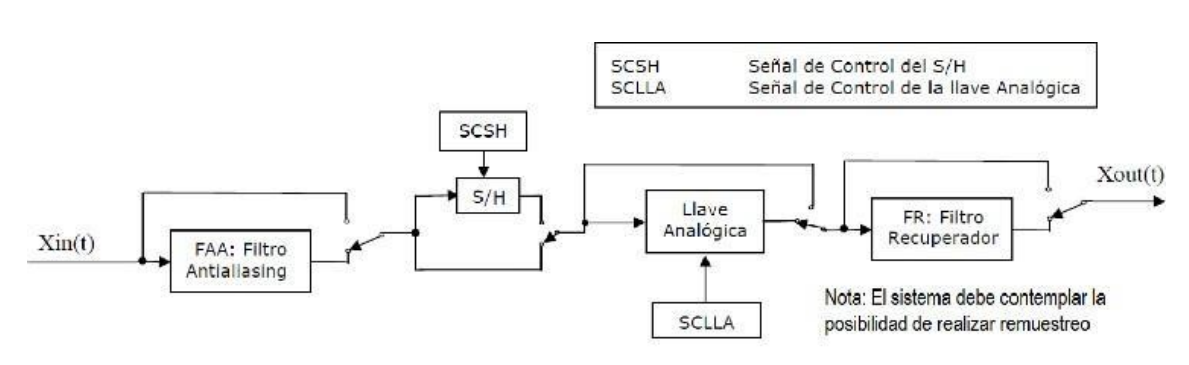
\includegraphics[width=0.8\textwidth]{Imagenes/Circuito_Muestreo.png}
    \caption{Circuito de Muestreo y Retención}
    \label{fig:Circuito_Muestreo}
\end{figure}
Esta implementación del circuito de muestreo y recuperación de la señal analógica nos permite analizar 
los efectos de las distintas etapas del proceso de muestreo y su importancia en el sampleo de la señal.

\subsection{Filtros Pasabajos}

La señal a muestrear que limita el diseño de los filtros corresponde 
a una onda cuadrada de amplitud $V_{\max}$, ciclo de trabajo $D = 0.75$ 
y período

\[
T = \frac{2}{f_i}, \quad f_i = 15 \,\text{kHz},
\]

de modo que la frecuencia fundamental resulta

\[
f_0 = \frac{1}{T} = \frac{f_i}{2} = 7.5 \,\text{kHz}.
\]



La serie de Fourier de una onda cuadrada con duty $D$ se obtiene a partir 
de los coeficientes

Consideremos una señal cuadrada periódica de amplitud $A$, periodo $T$ y duty cycle $D$:

\[
x(t) =
\begin{cases}
A, & 0 \le t < D T \\
0, & D T \le t < T
\end{cases}
\]

y se repite cada $T$ segundos.
Los coeficientes de la serie de Fourier están dados por:

\[
c_n = \frac{1}{T} \int_0^T x(t) e^{-j n \omega_0 t} dt, \quad \omega_0 = \frac{2 \pi}{T}
\]

Para nuestra señal cuadrada:

\[
c_n = \frac{1}{T} \int_0^{D T} A e^{-j n \omega_0 t} dt
= \frac{A}{T} \int_0^{D T} e^{-j n \omega_0 t} dt
\]

Integrando:

\[
c_n = \frac{A}{T} \left[ \frac{e^{-j n \omega_0 t}}{-j n \omega_0} \right]_0^{D T}
= \frac{A}{j n \omega_0 T} \left( 1 - e^{-j n \omega_0 D T} \right)
\]

Como $\omega_0 T = 2 \pi$:

\[
c_n = \frac{A}{j 2 \pi n} \left( 1 - e^{-j 2 \pi n D} \right), \quad n \neq 0
\]

Para $n = 0$ (componente DC):

\[
c_0 = \frac{1}{T} \int_0^T x(t) dt = \frac{A \cdot D T}{T} = A D
\]



Usando la identidad $1 - e^{-j \theta} = 2 j \sin(\theta/2) e^{-j \theta/2}$, la magnitud de cada armónico es:

\[
|c_n| = \frac{A}{n \pi} \left| \sin(n \pi D) \right|
\]

- Para $D = 0.75$:

\[
|c_n| = \frac{A}{n \pi} \left| \sin(0.75 \, n \pi) \right|
\]

Ya que para una buena reconstruccion de la misma es necesario que los filtros
capturen la mayor cantidad de harmónicos posibles, se decidio colocar
la frecuencia de corte en $f_c = 80 \,\text{kHz}$, lo cual permite capturar 
hasta 10 harmónicos (no nulos) de la señal de entrada.

Para el diseño de los filtros se utilizo la aproximación de Cauer (elíptica), 
con 3 celdas Sedra colocadas en cascada.

\subsection{Oscilador}

\subsection{Obtención de Señal Muestreada}



%---------------- 3da Seccion ----------------%
\section{Filtros Pasa Bajos}
\begin{figure}[H]
    \centering
    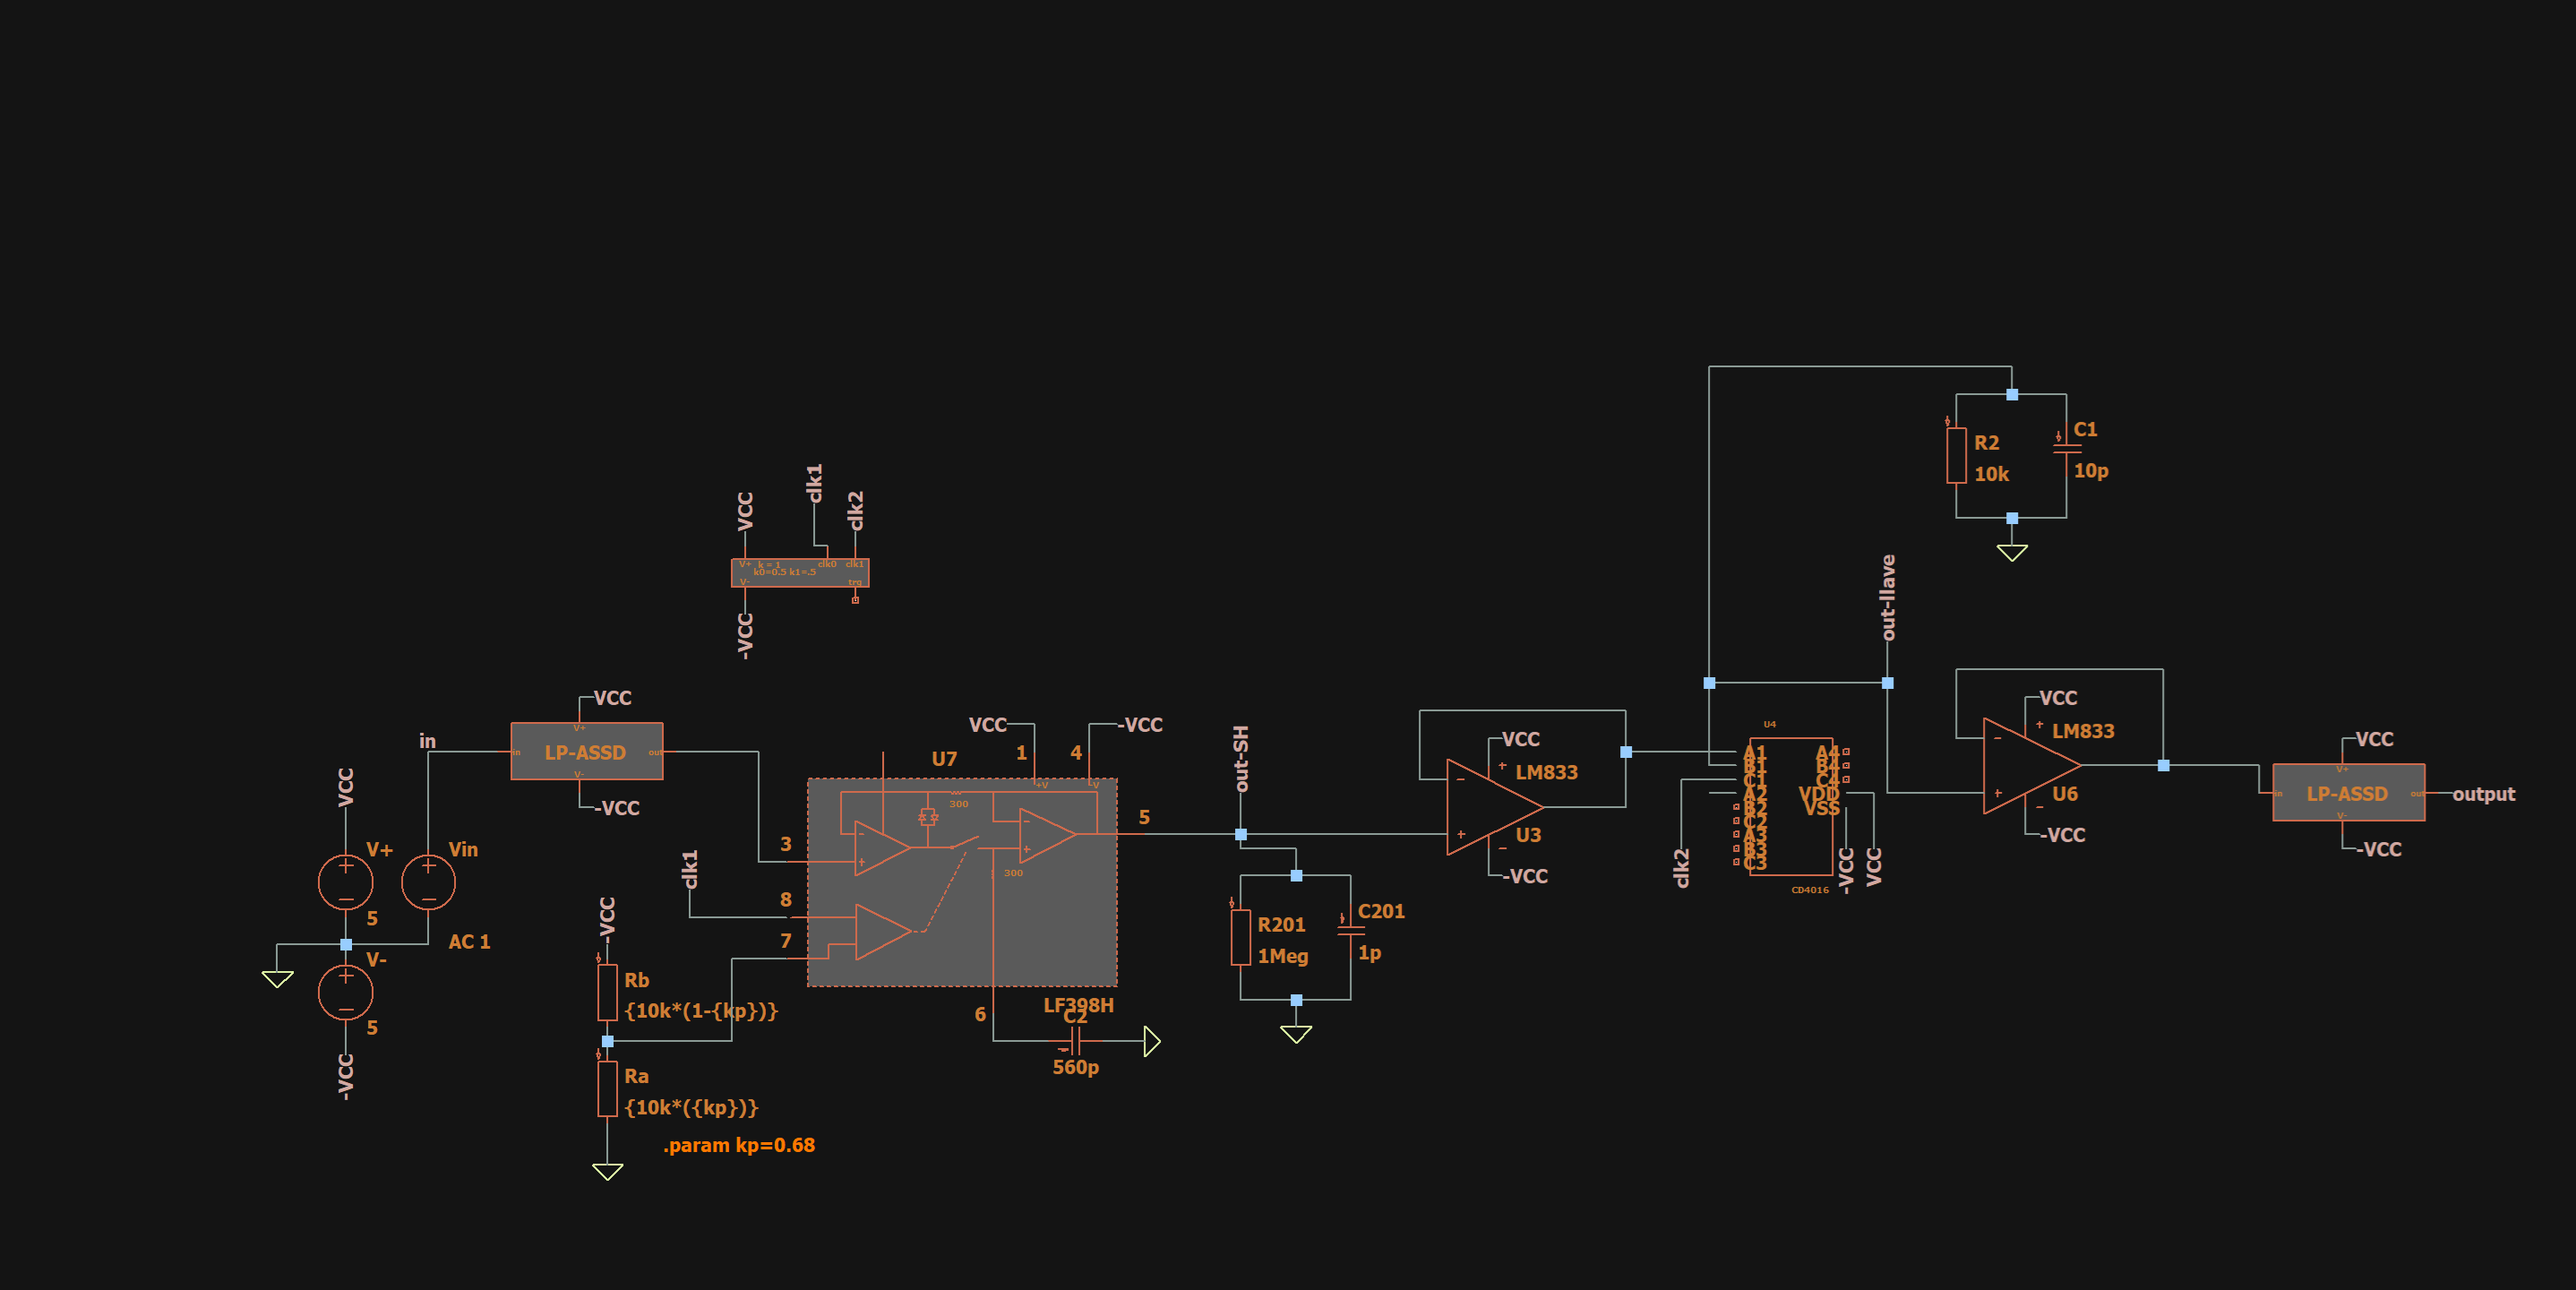
\includegraphics[width=0.9\linewidth]{Imagenes Nacho/EsquemaLatex.png}
    \caption{Circuito completo de simulaci\'on en LTSpice}
    \label{fig:EsquemaLatex}
\end{figure}


Para garantizar el correcto funcionamiento del circuito, se opt\'o por simular por m\'odulos el circuito, creando componentes de los mismos una vez que su funcionamiento era reconocido para un esquema final como se observa en la figura \ref{fig:EsquemaLatex} . 

\subsection{Filtro Low-Pass}
El componente "LP-ASSD", encapsula un filtro pasabajos de 6to orden Cauer con frecuencia de corte en $80kHz$. Se decidi\'o por 3 celdas SEDRA en cascada, debido a su facilidad de implementaci\'on y experiencia previa con los mismos. Luego de encontrar los polos y zeros de cada celda y evaluar las etapas de ganancia para evitar saturaci\'on entre etapas, se simul\'o el orden y condiciones de las mismas para garantizar su funcionamiento optimo. A continuaci\'on los resultados:

\begin{figure}[H]
    \centering
    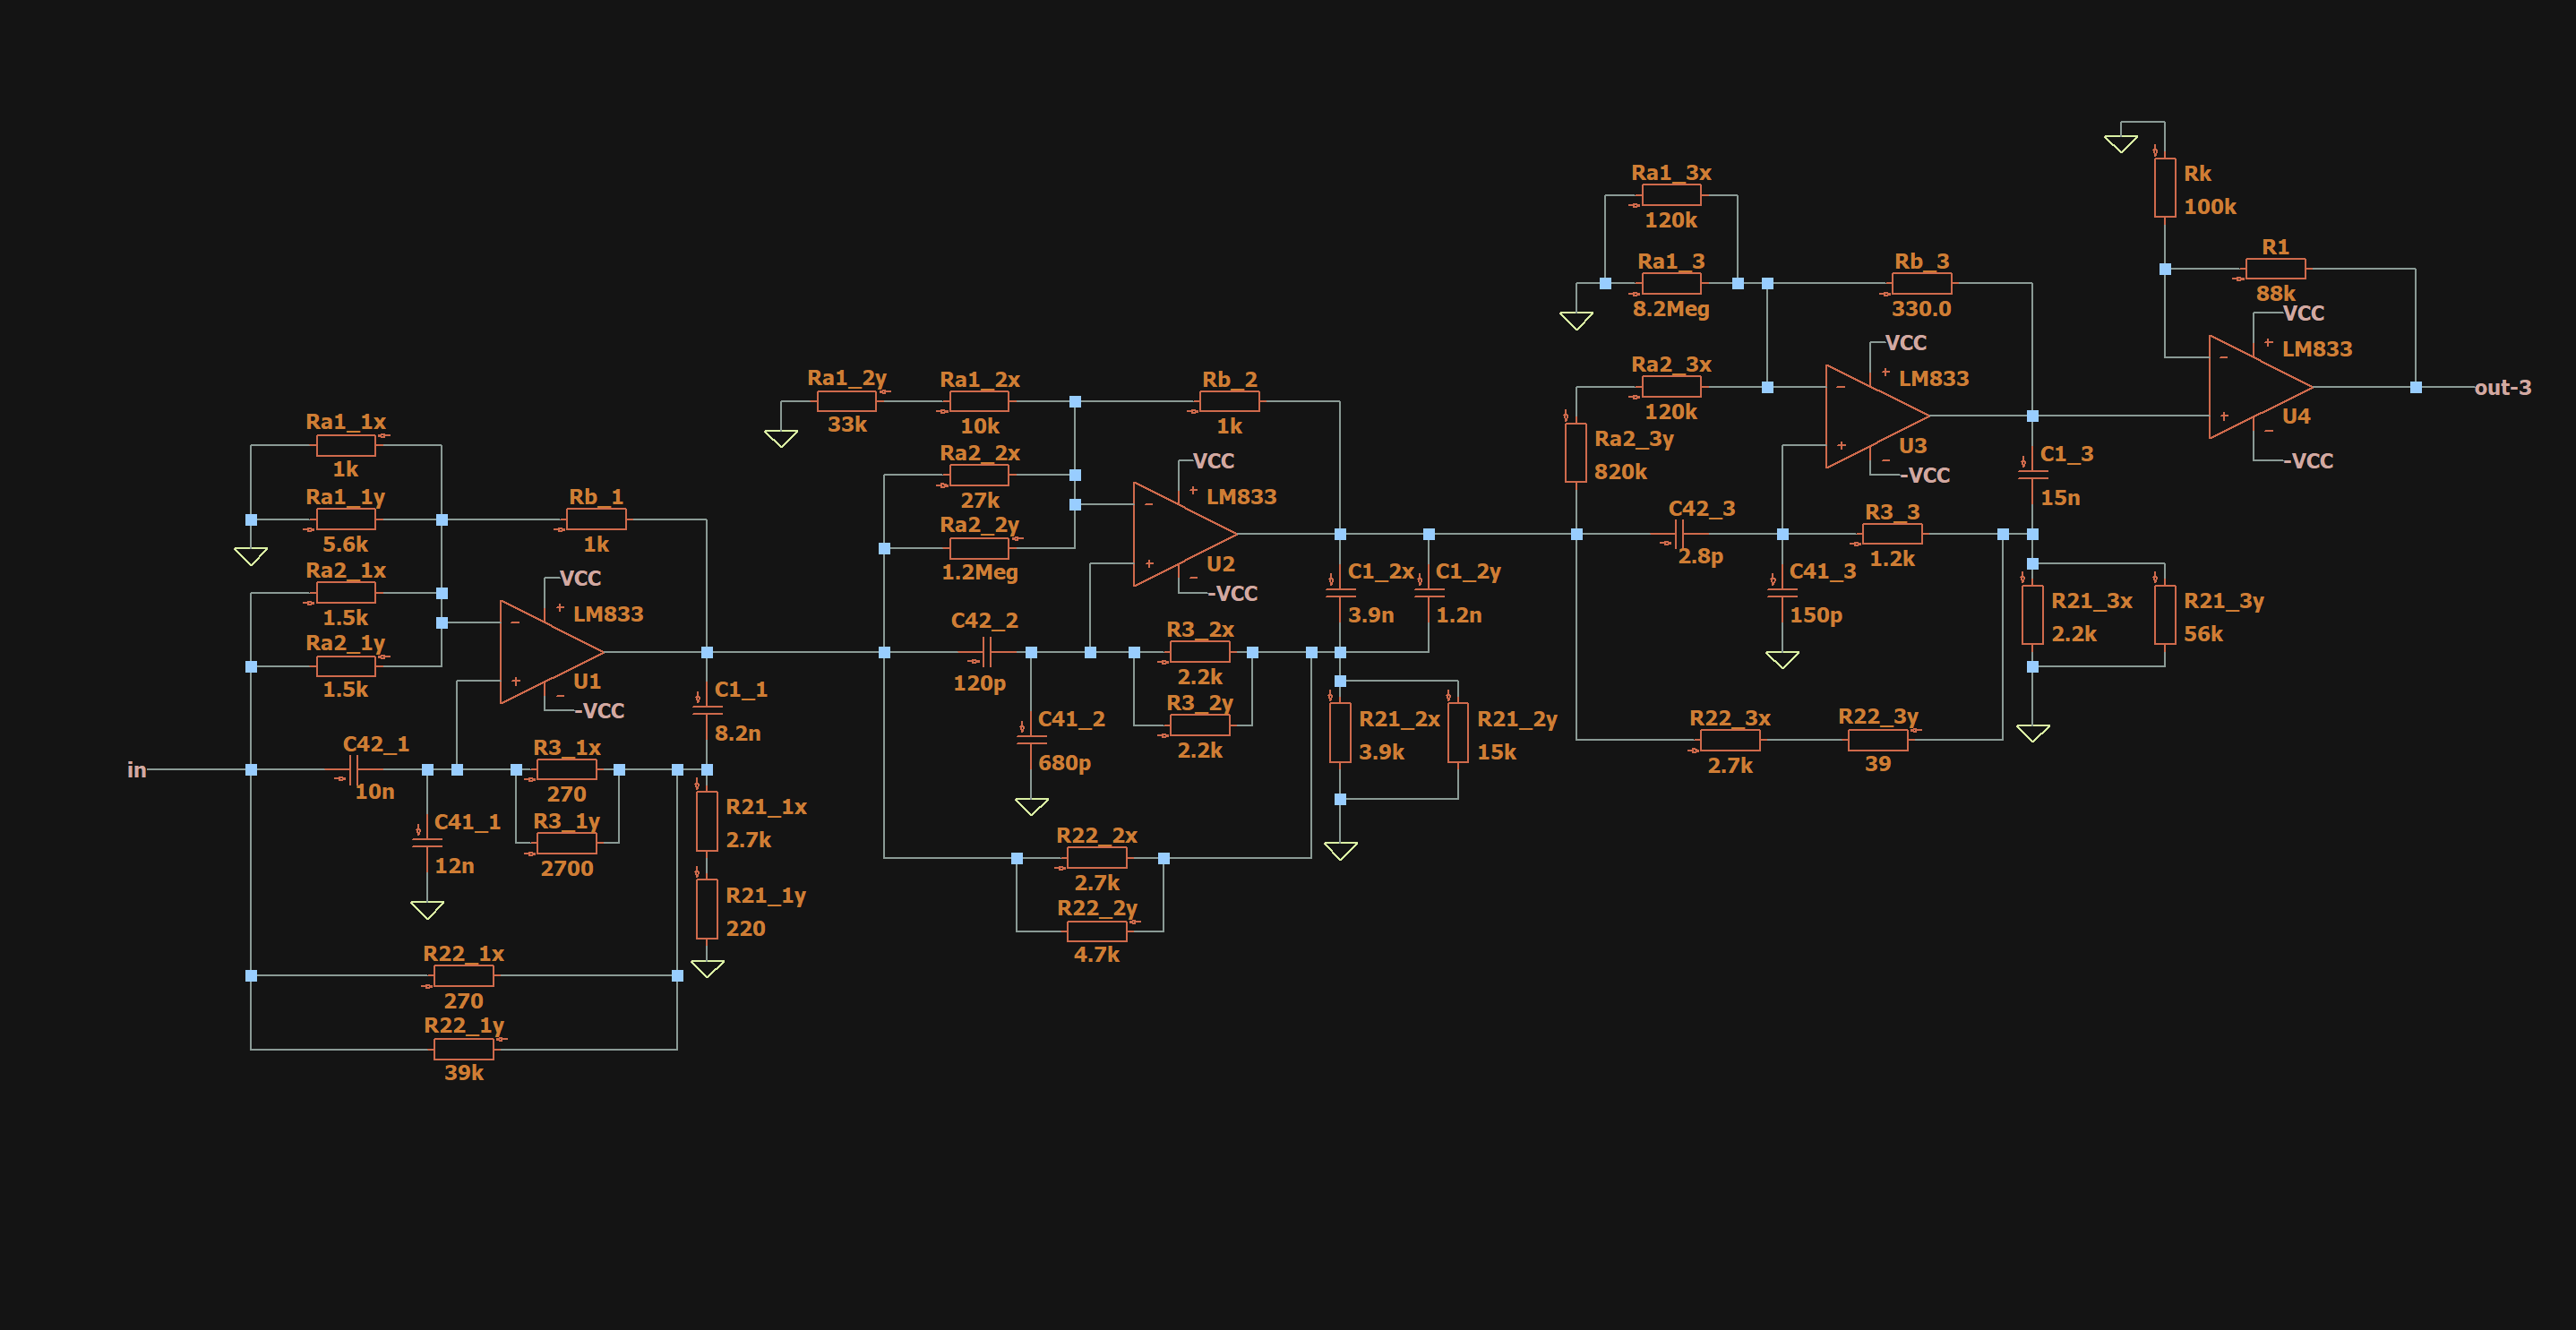
\includegraphics[width=0.8\linewidth]{Imagenes Nacho/EsquemaLatexLowPass.png}
    \caption{Celdas SEDRA en cascada como filtros Low-Pass}
    \label{fig:EsquemaLatexLowPass}
\end{figure}

\begin{figure}[H]
    \centering
    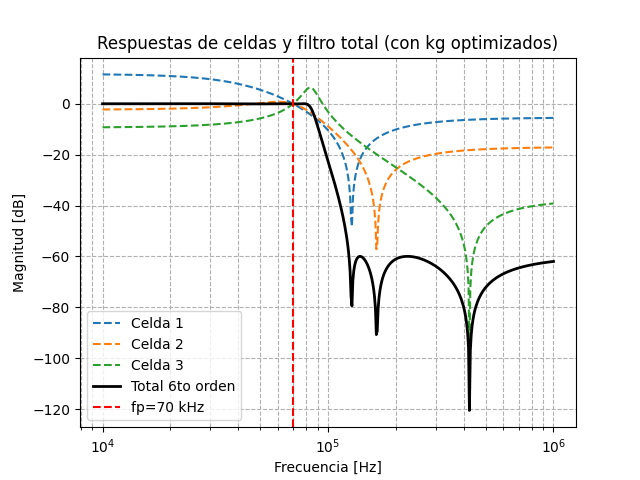
\includegraphics[width=0.8\linewidth]{Imagenes Nacho/Python.png}
    \caption{Evaluaci\'on de Etapas de Celdas Individuales}
    \label{fig:Python}
\end{figure}

\begin{figure}[H]
    \centering
    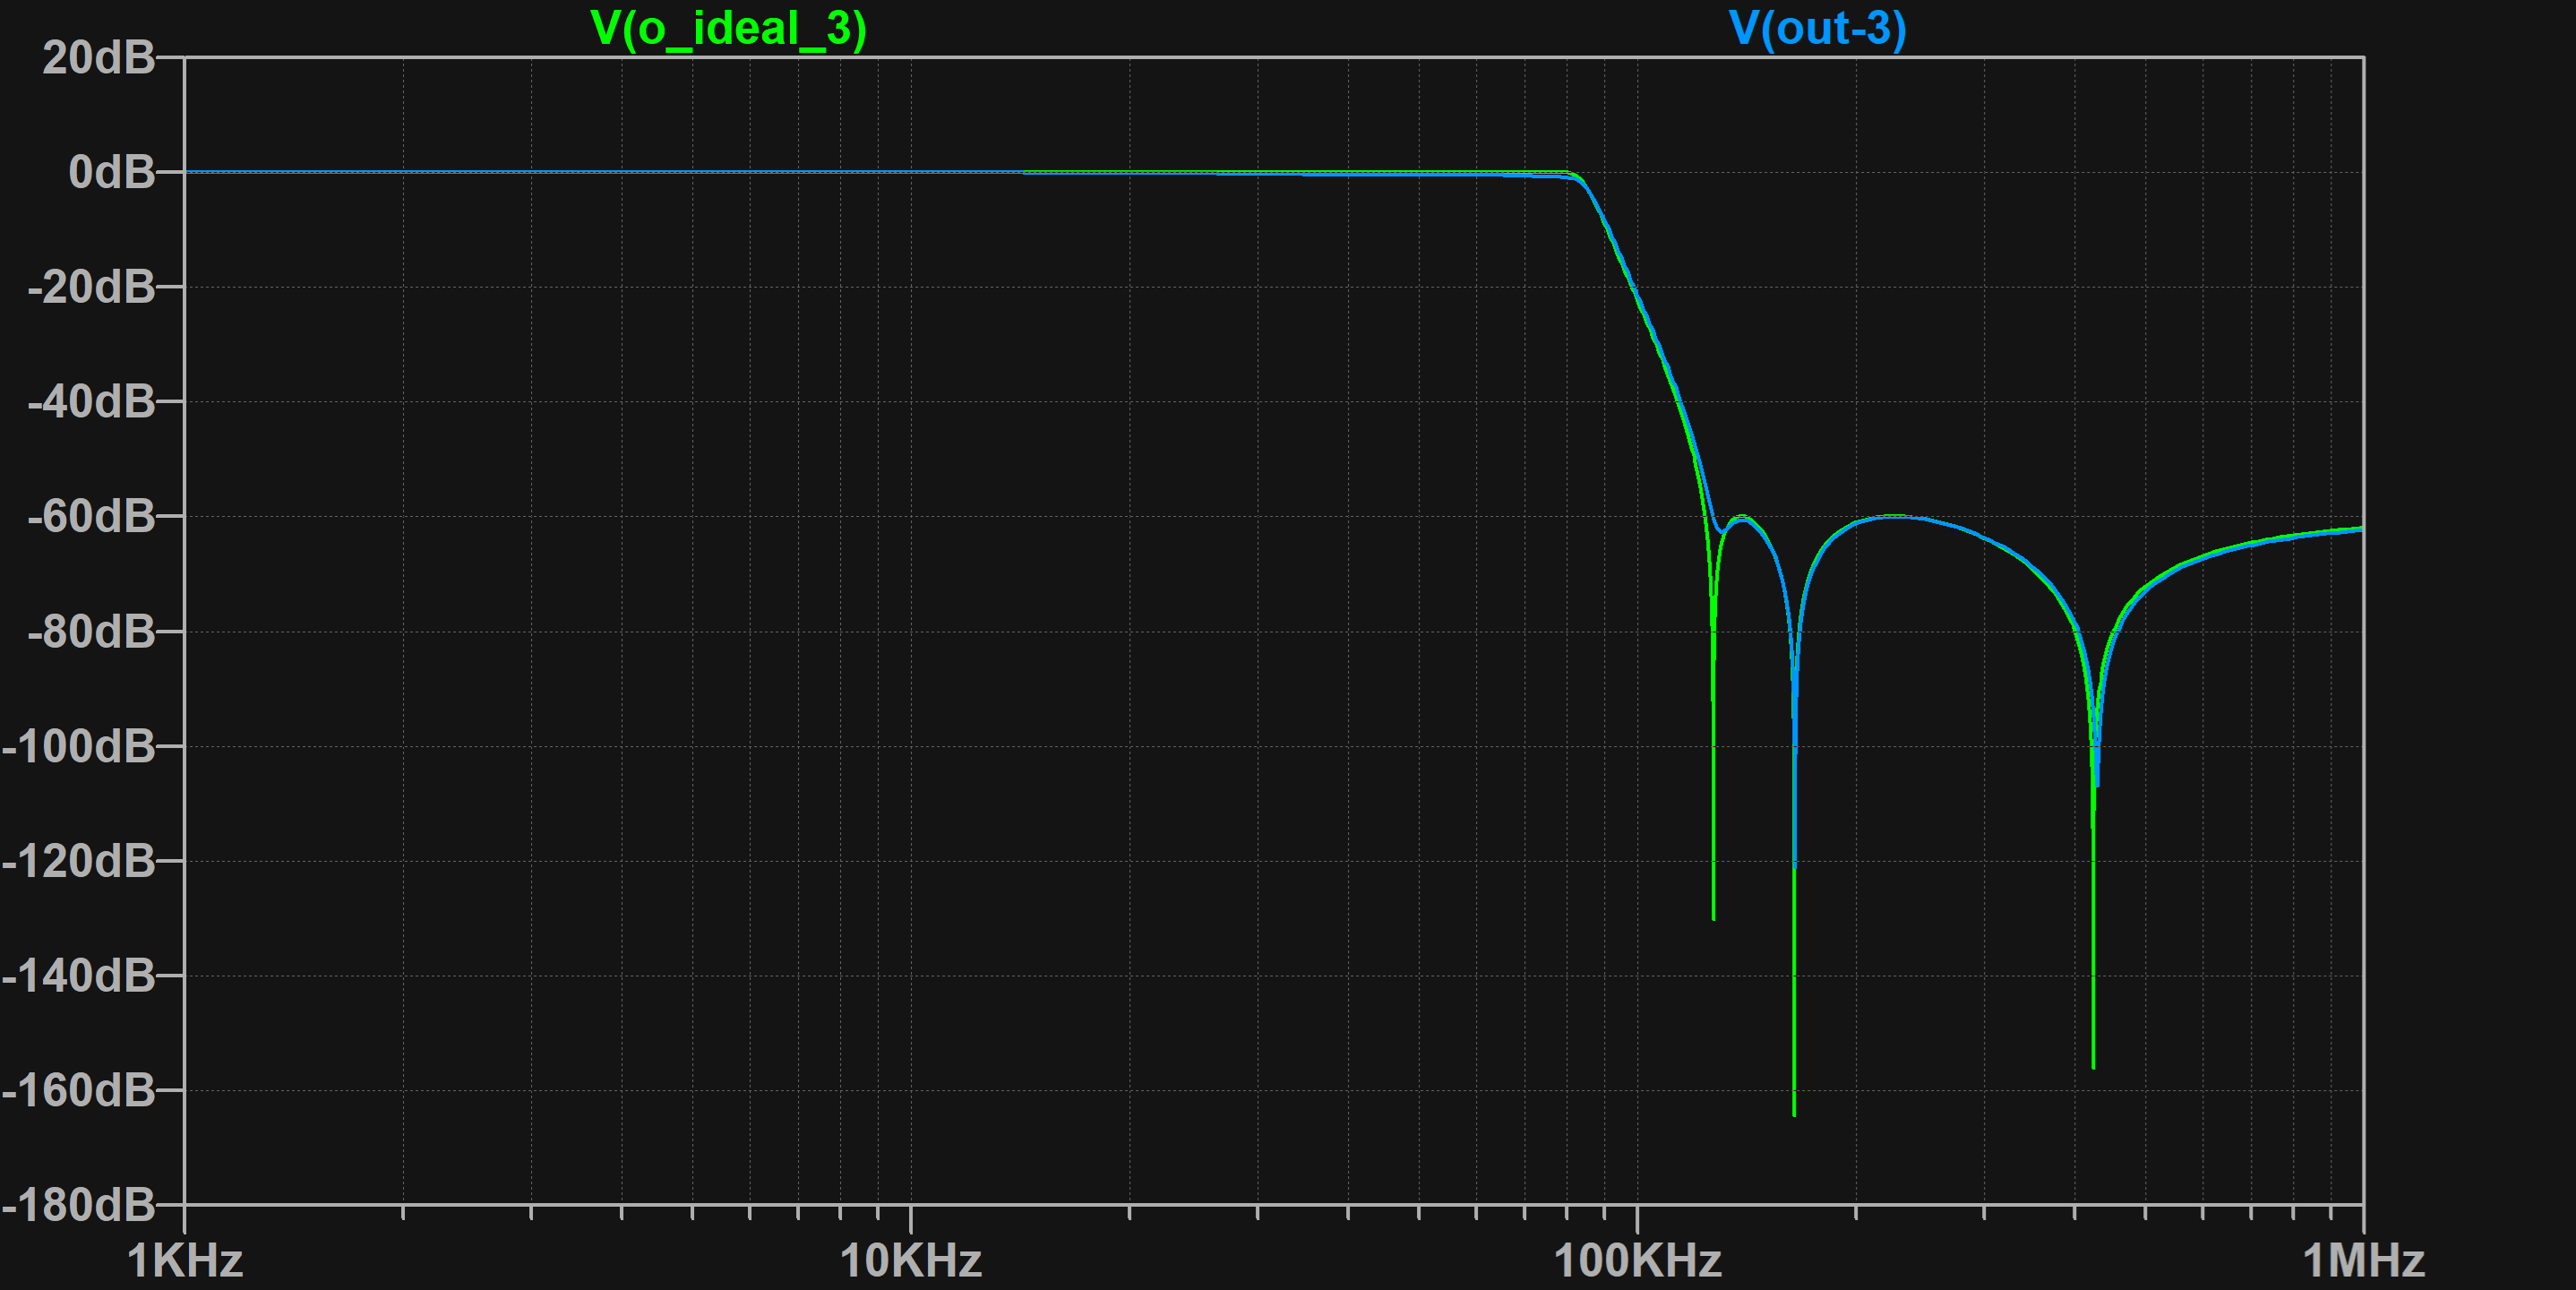
\includegraphics[width=0.8\linewidth]{Imagenes Nacho/LowPassFitler.png}
    \caption{Filtro Low Pass: Funci\'on ideal vs Implentacion}
    \label{fig:LowPassFitler}
\end{figure}

un problema que tuvo este filtro en su implementaci\'on, es que la primera etapa posee una impedancia de entrada muy, por lo que se debi\'o colocar un buffer. Adem\'as, La ganacia en la vida real se desvia de la expectativa por las tolerancias de los componentes, por lo que se debe colocar una etapa de ganancia variable para garantizar que no se atenuen las frecuencias deseadas.

\subsection{Oscilador}

El pequeño componente que se puede apreciar en la figura \ref{fig:EsquemaLatex}, encapsula el circuito generador de clock. El mismo requiere unicamente como entrada las fuentes de alimentaci\'on, con las salidas siendo la carga y descarga de un capacitor ($trg$), clock 1($clk1$) y clock 1($clk2$). Variando $k$ se ajusta la frecuencia de los clocks podiendo llegar hasta los $250kHz$ y ajustando $k1$ y $k2$ el duty de los respectivos clocks. 

\begin{figure}[H]
    \centering
    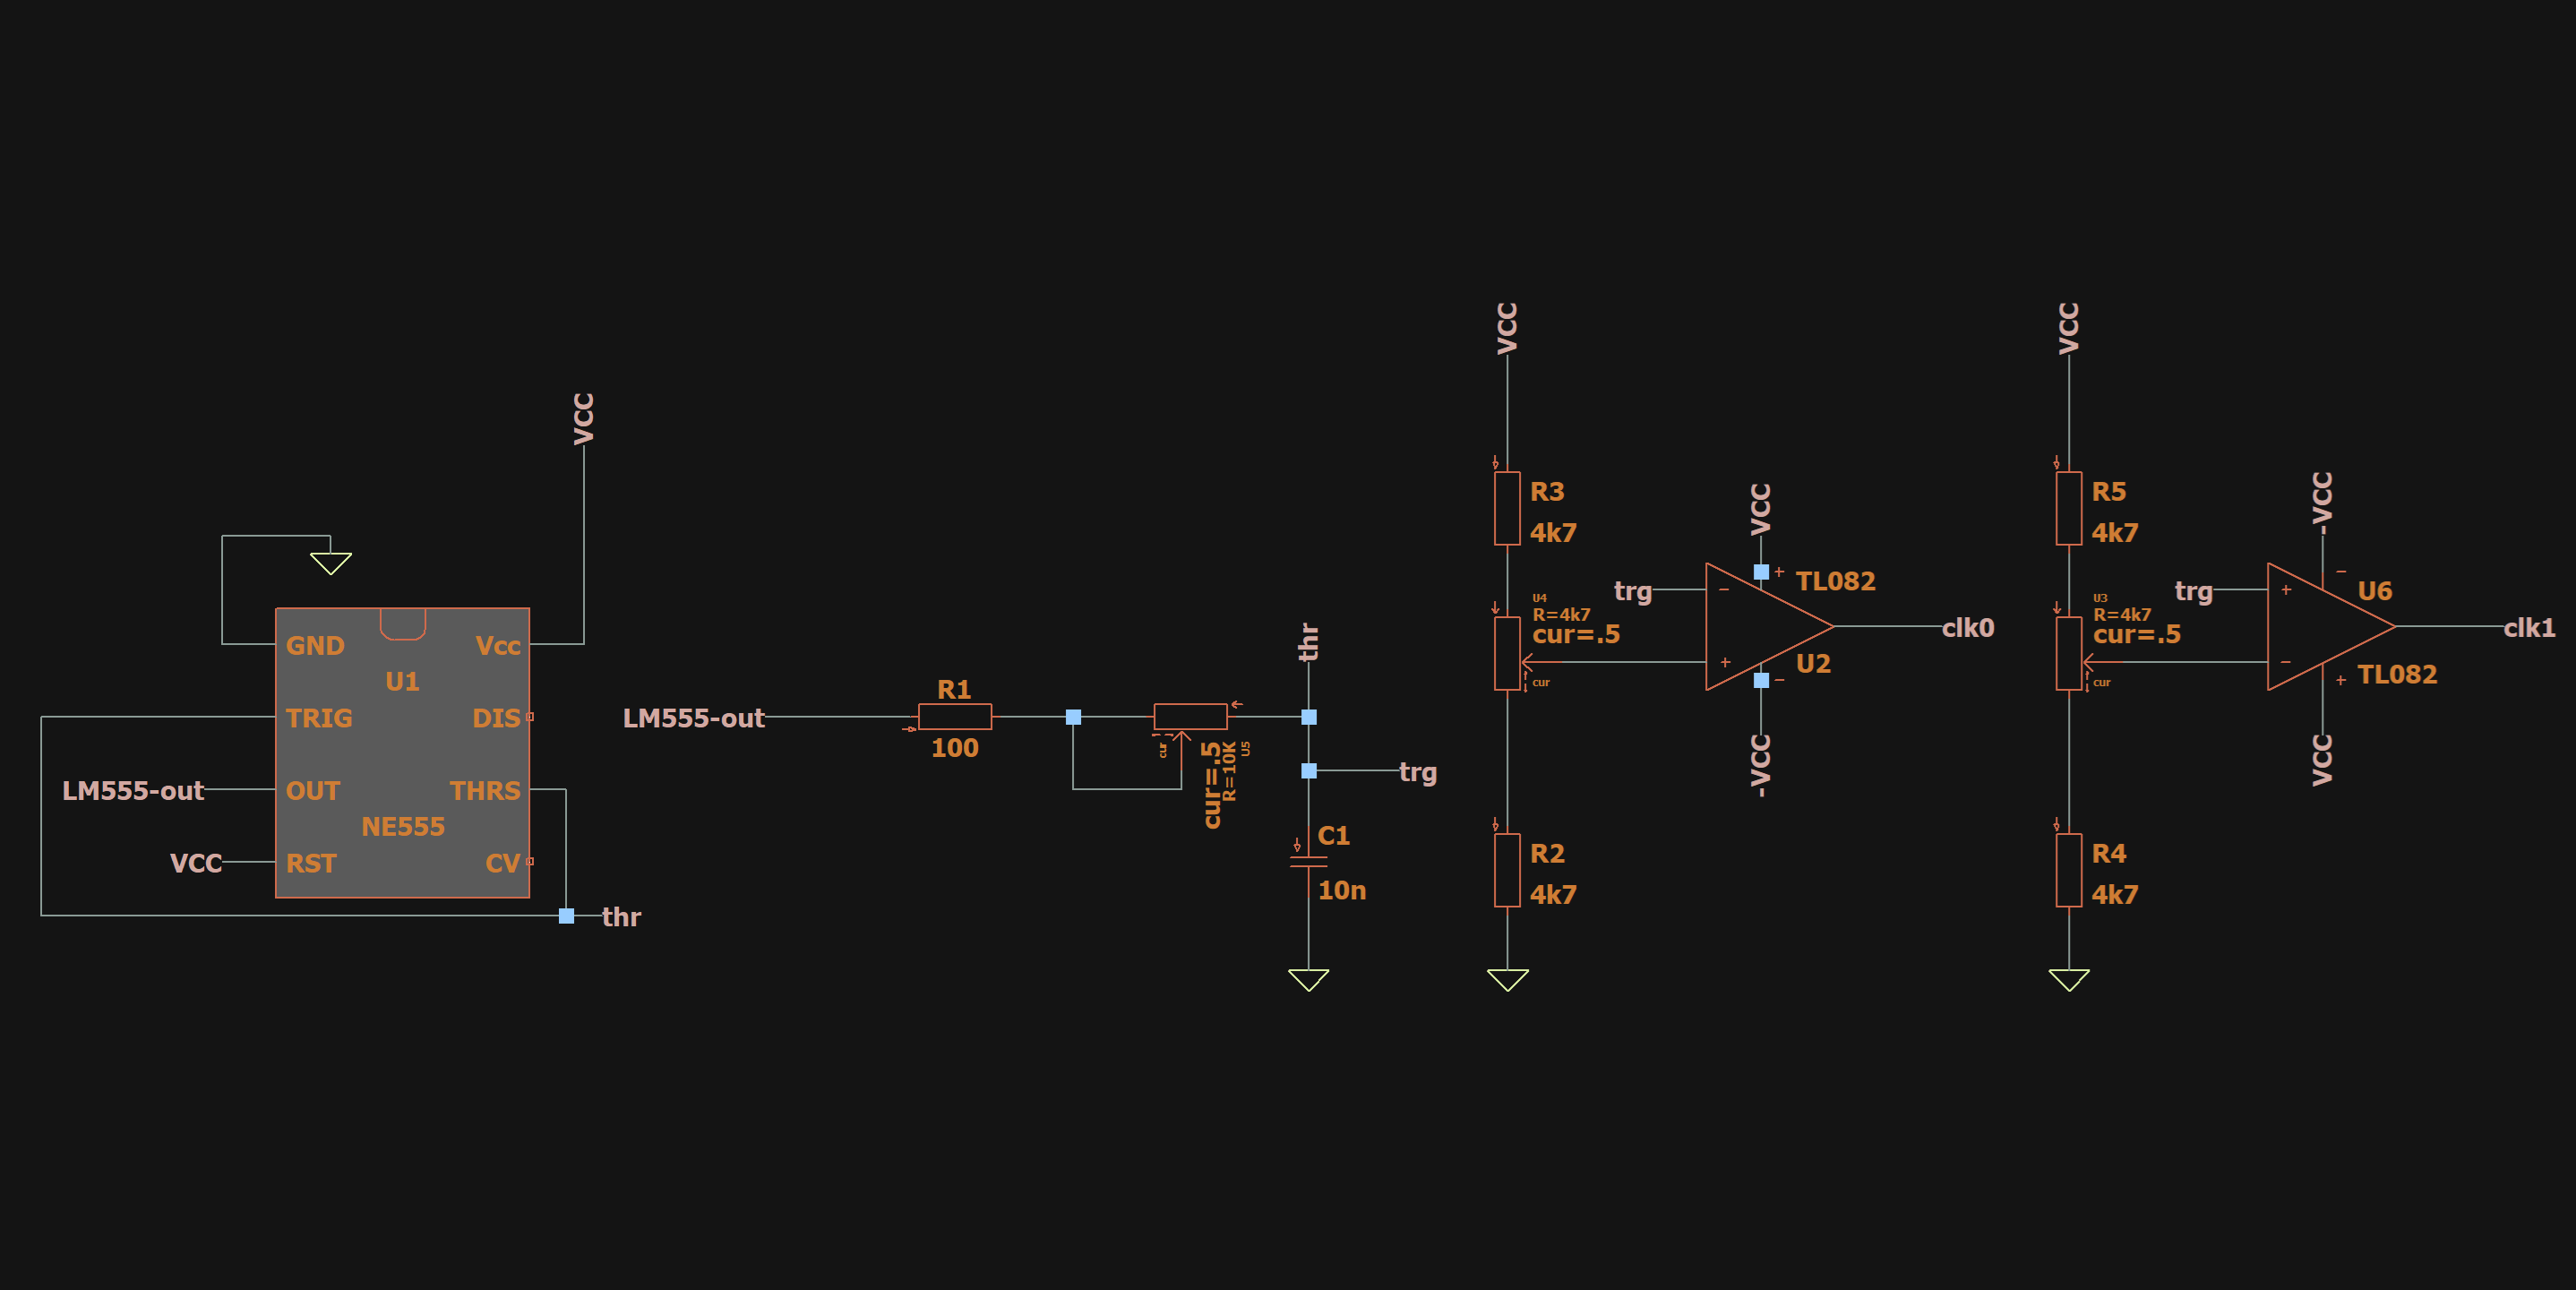
\includegraphics[width=0.8\linewidth]{Imagenes Nacho/OsciladorEsquema.png}
    \caption{Clocks del Sistema}
    \label{fig:OsciladorEsquema}
\end{figure}

\begin{figure}[H]
    \centering
    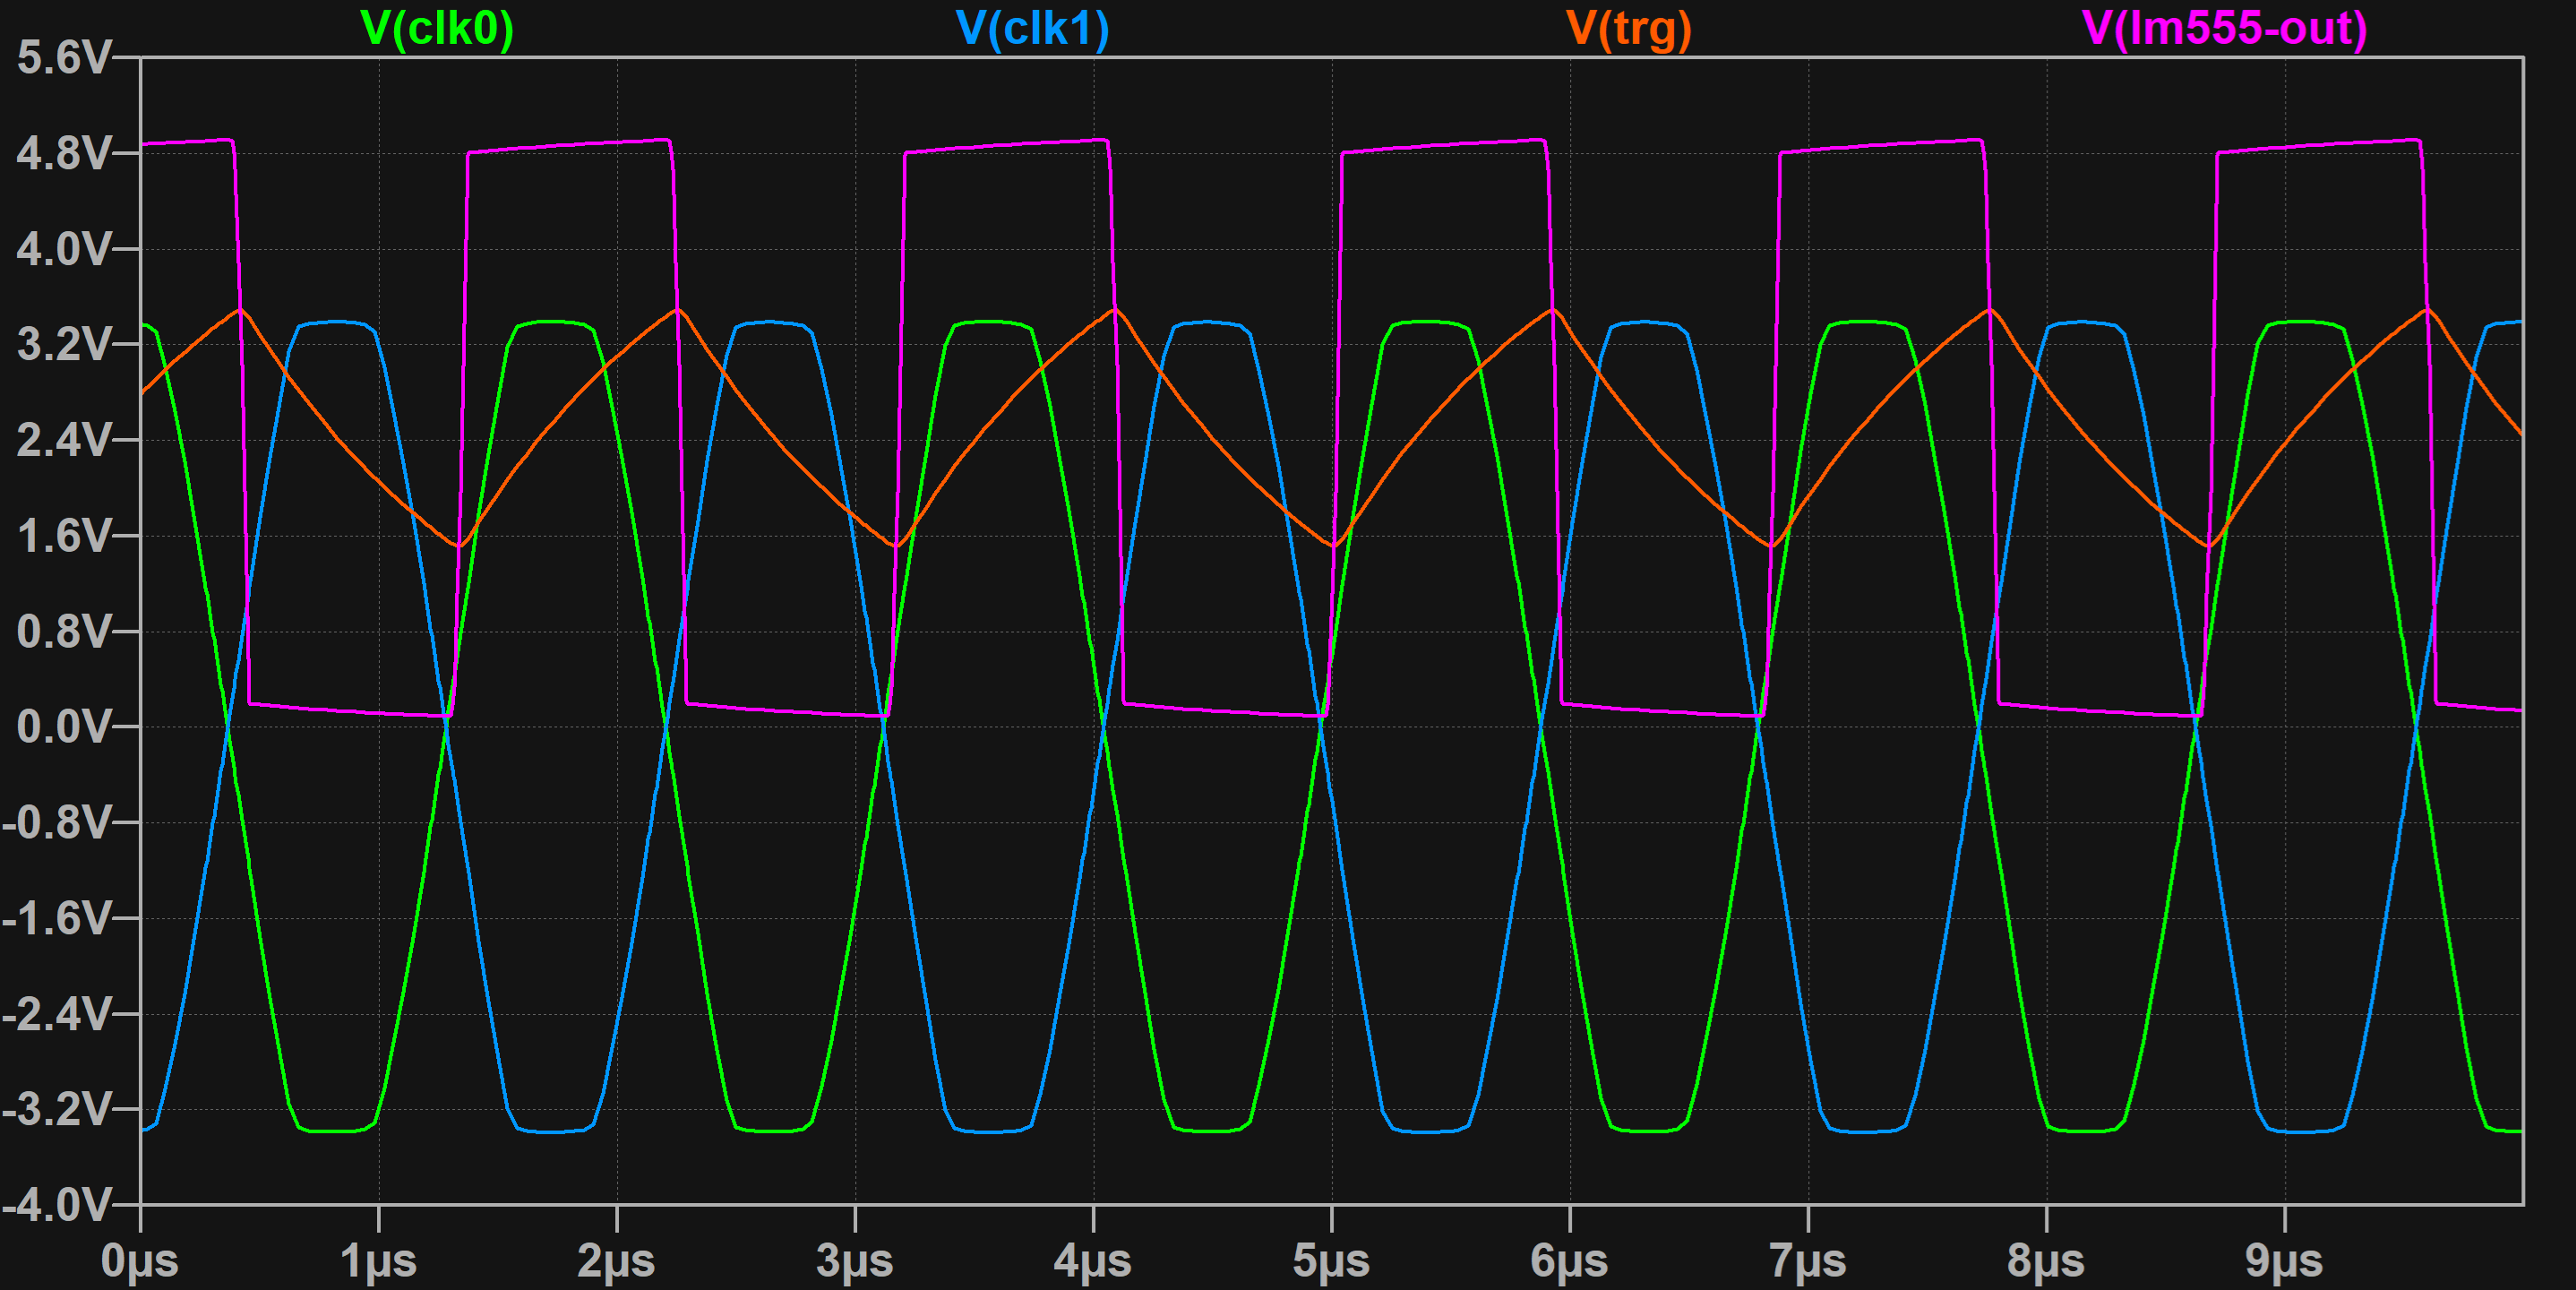
\includegraphics[width=0.8\linewidth]{Imagenes Nacho/Oscilador.png}
    \caption{Simulaci\'on de clock $250kHz$}
    \label{fig:Oscilador}
\end{figure}

\subsection{Simulaci\'on de Muestro Natural}
Muestreando una señal cuadrada de $f = 15kHz$ con $75\%$ de Duty Cycle a $f_s = 250kHz$ obtenemos los siguientes graficos:

\begin{figure}[H]
    \centering
    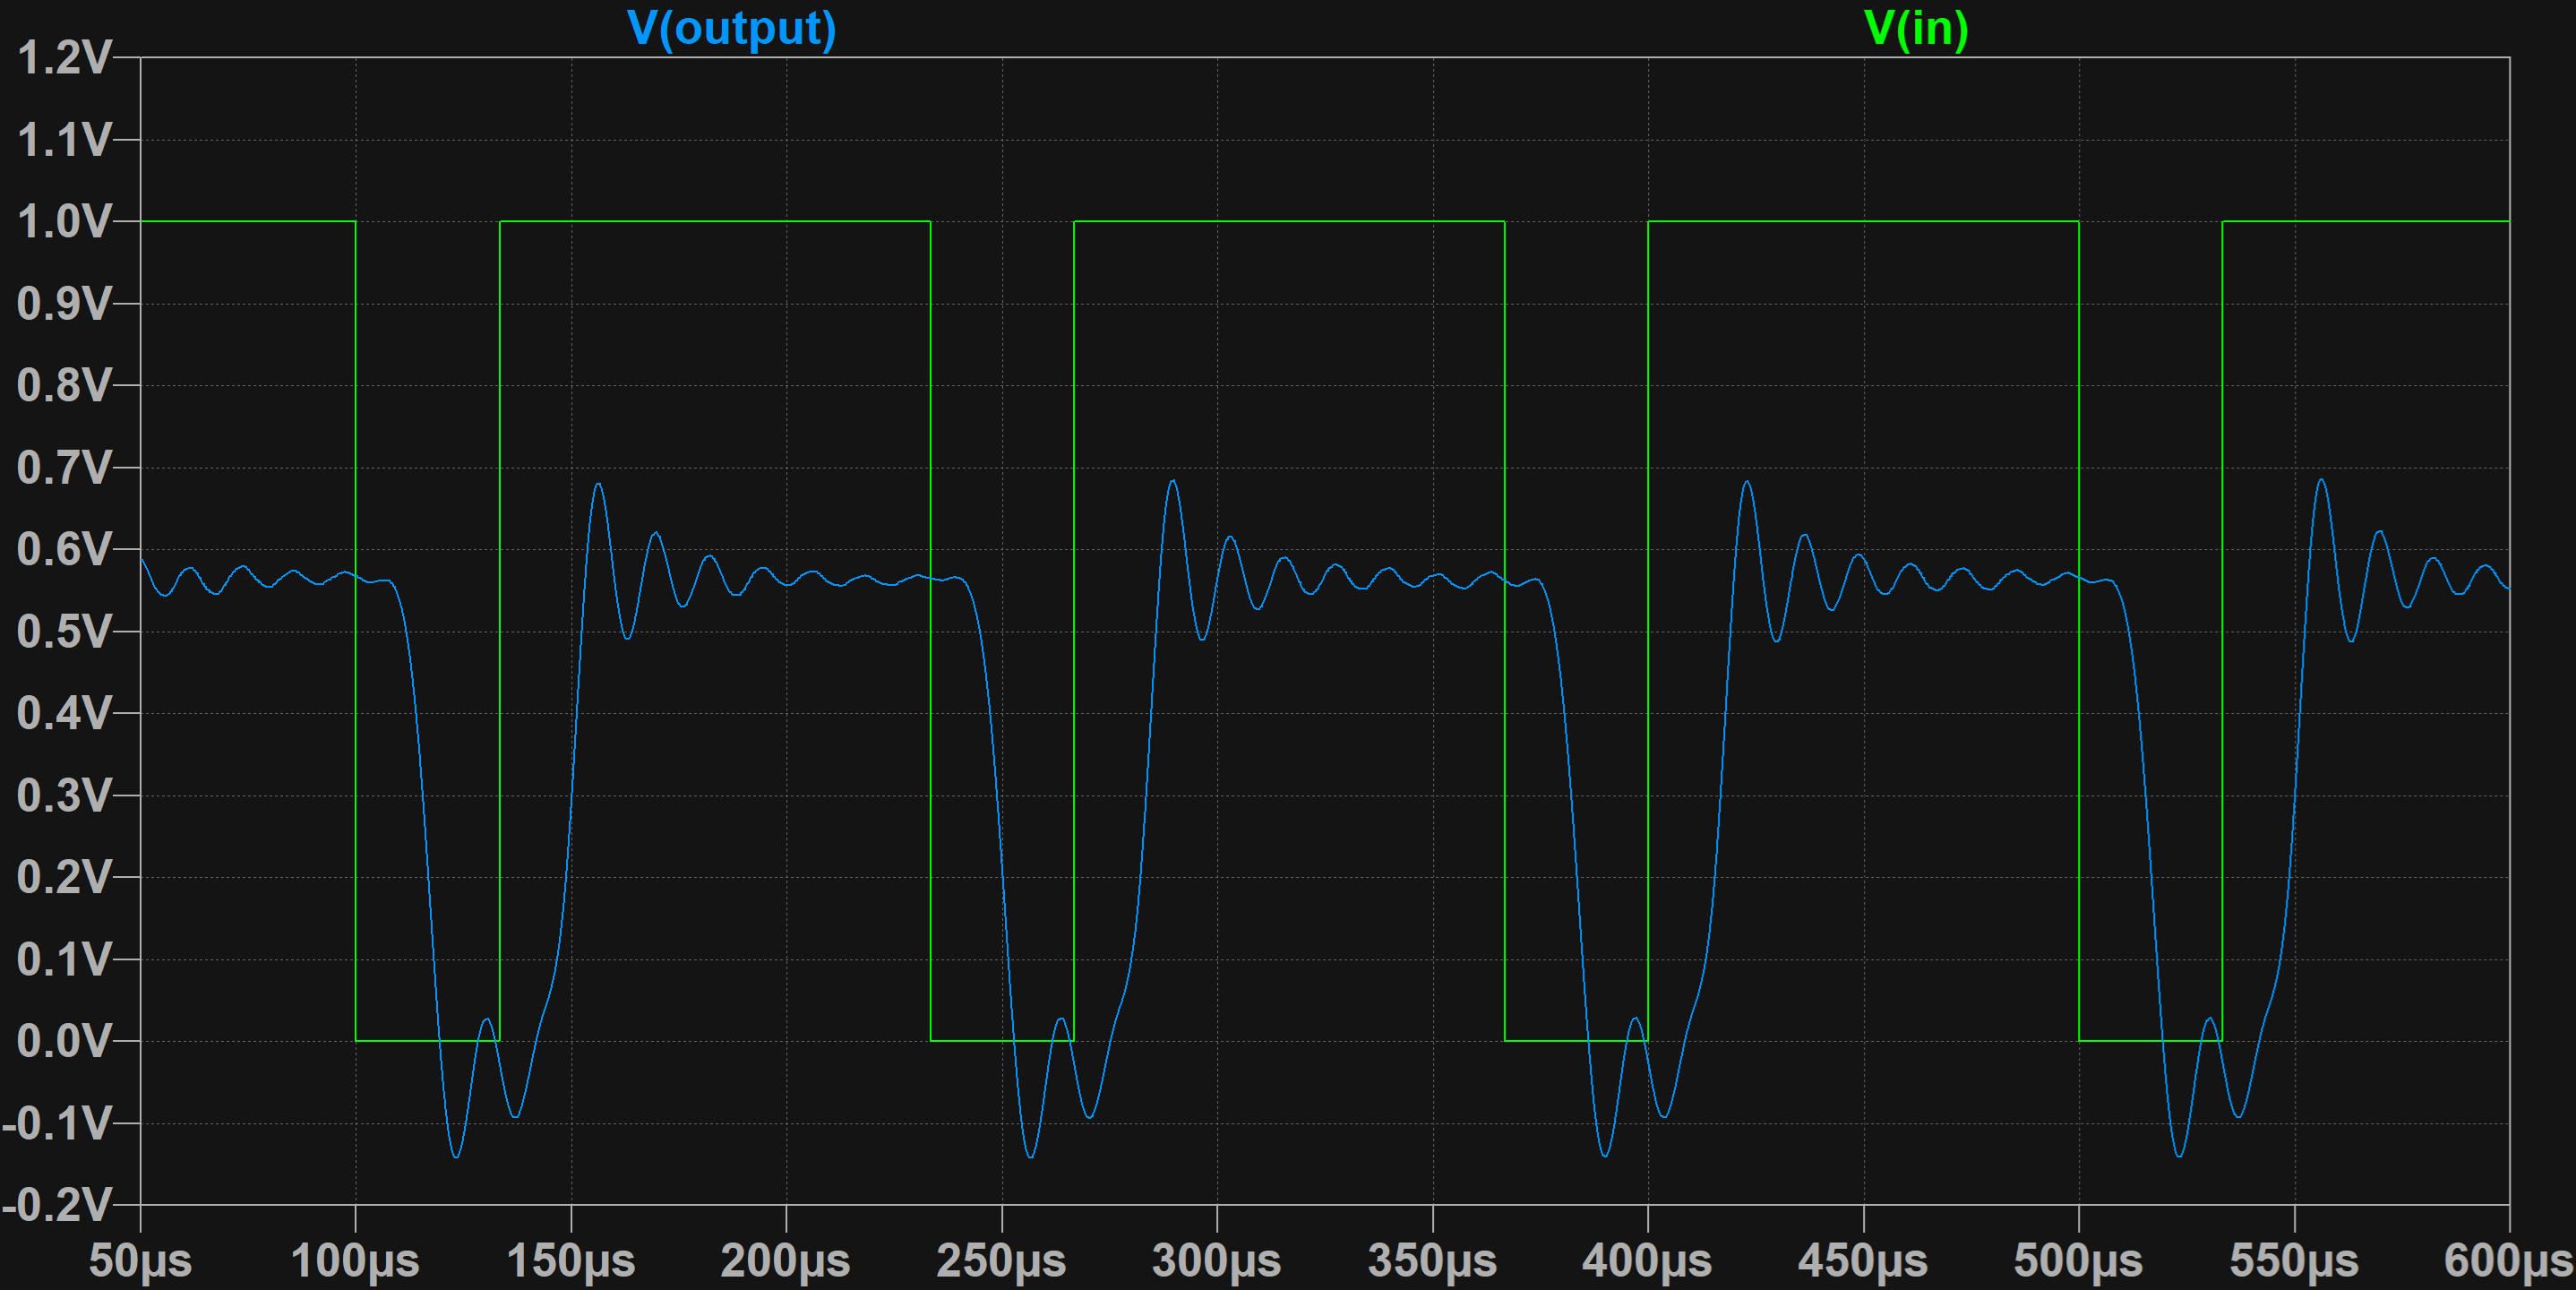
\includegraphics[width=0.8\linewidth]{Imagenes Nacho/Natural/Natural-Vi-Sqr15k.png}
    \caption{$V_o$ vs $V_i$}
    \label{fig:Natural-Vi-Sqr15k}
\end{figure}

\begin{figure}[H]
    \centering
    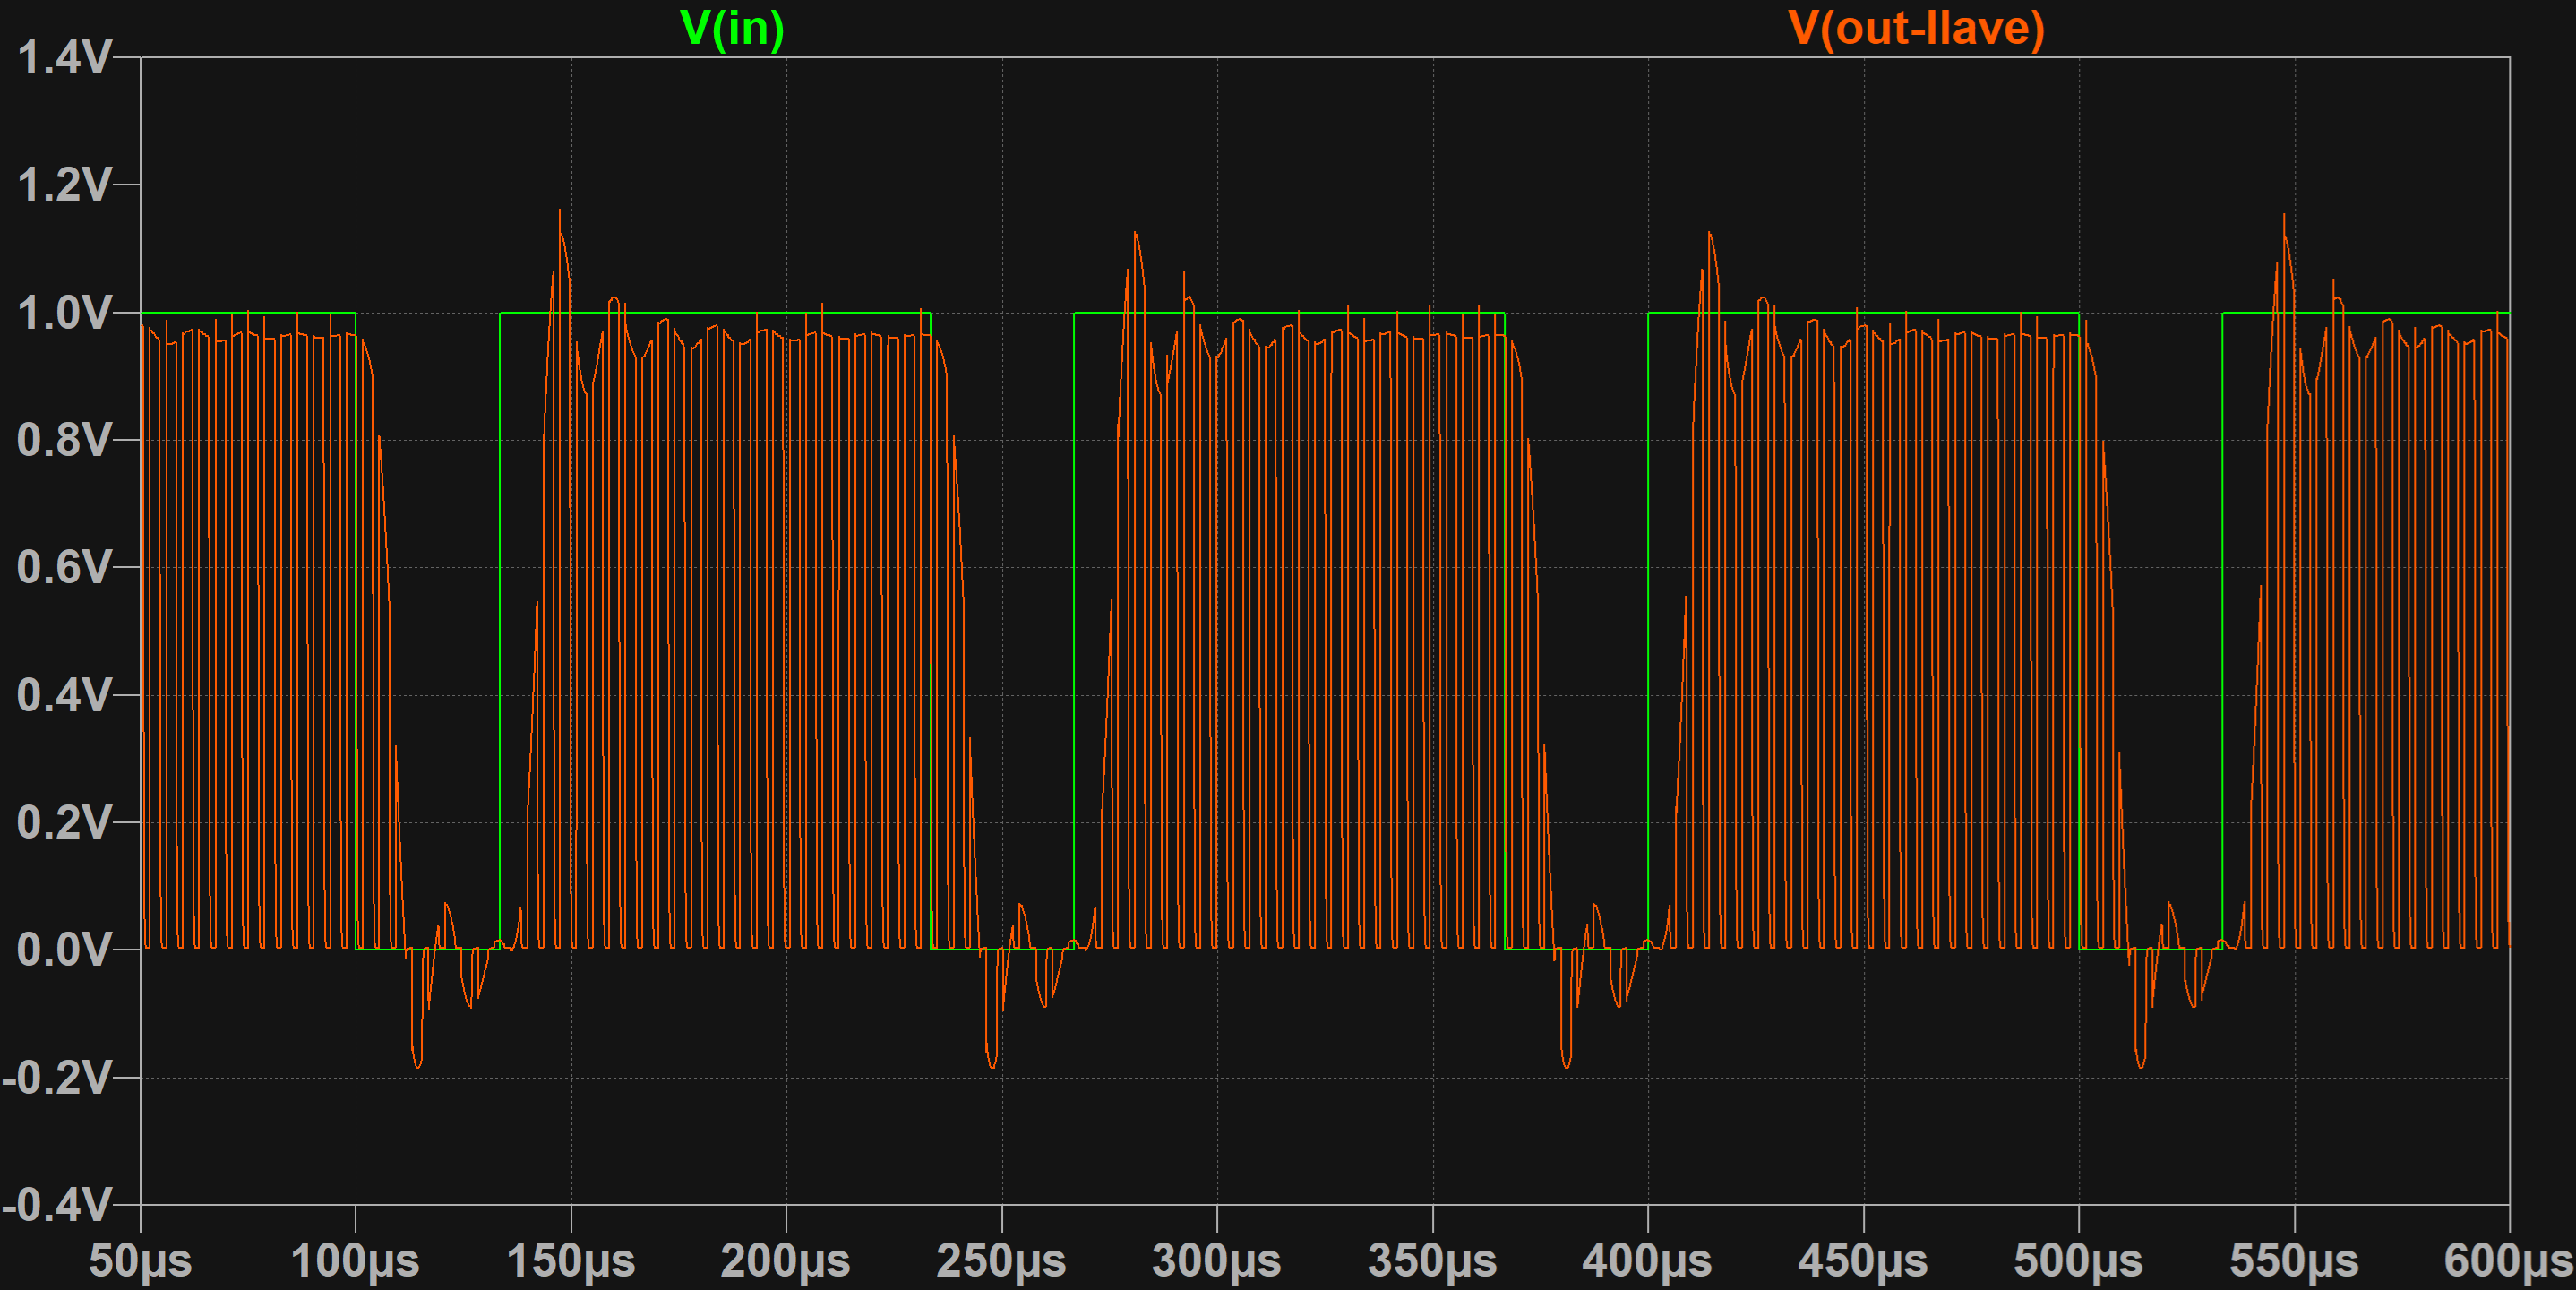
\includegraphics[width=0.8\linewidth]{Imagenes Nacho/Natural/Natural-Vi-Sqr15k-out-LLave.png}
    \caption{Salida de la llave vs $V_i$}
    \label{fig:out-LLave}
\end{figure}

\begin{figure}[H]
    \centering
    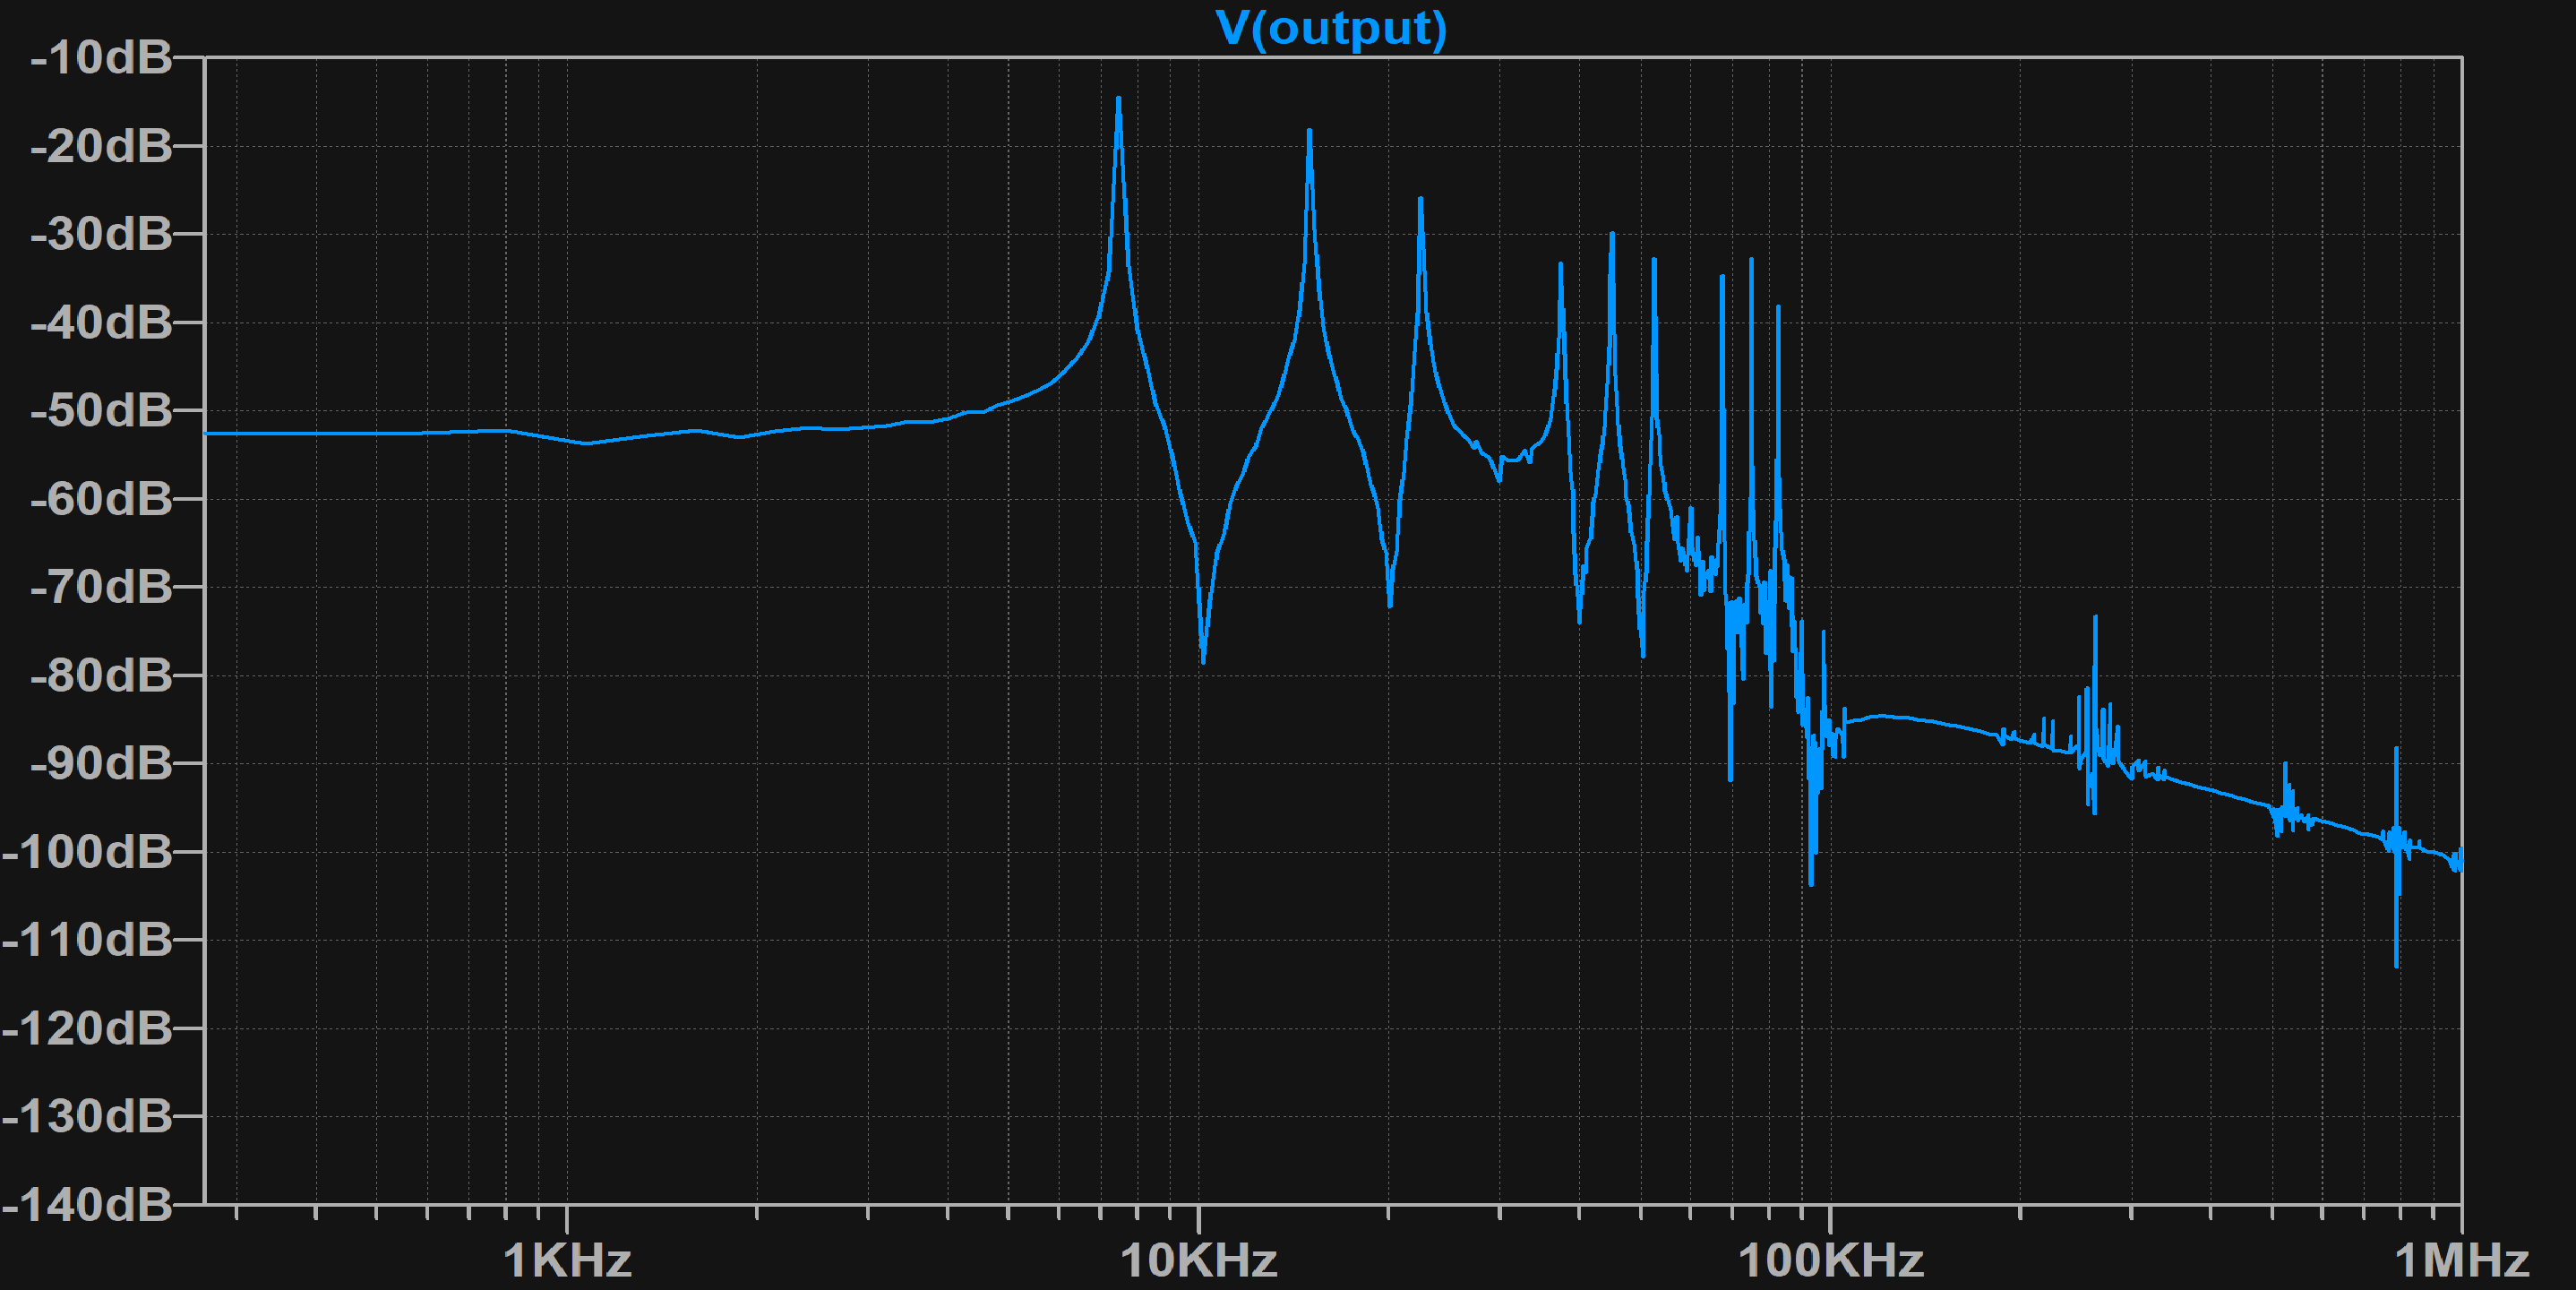
\includegraphics[width=0.8\linewidth]{Imagenes Nacho/Natural/Natural-Vi-Sqr15k-outFFT.png}
    \caption{FFT de la salida}
    \label{fig:FFT de la salida}
\end{figure}


\subsection{Simulaci\'on de Muestro Instantaneo}
Muestreando una señal cuadrada de $f = 15kHz$ con $75\%$ de Duty Cycle a $f_s = 250kHz$ obtenemos los siguientes graficos:

\begin{figure}[H]
    \centering
    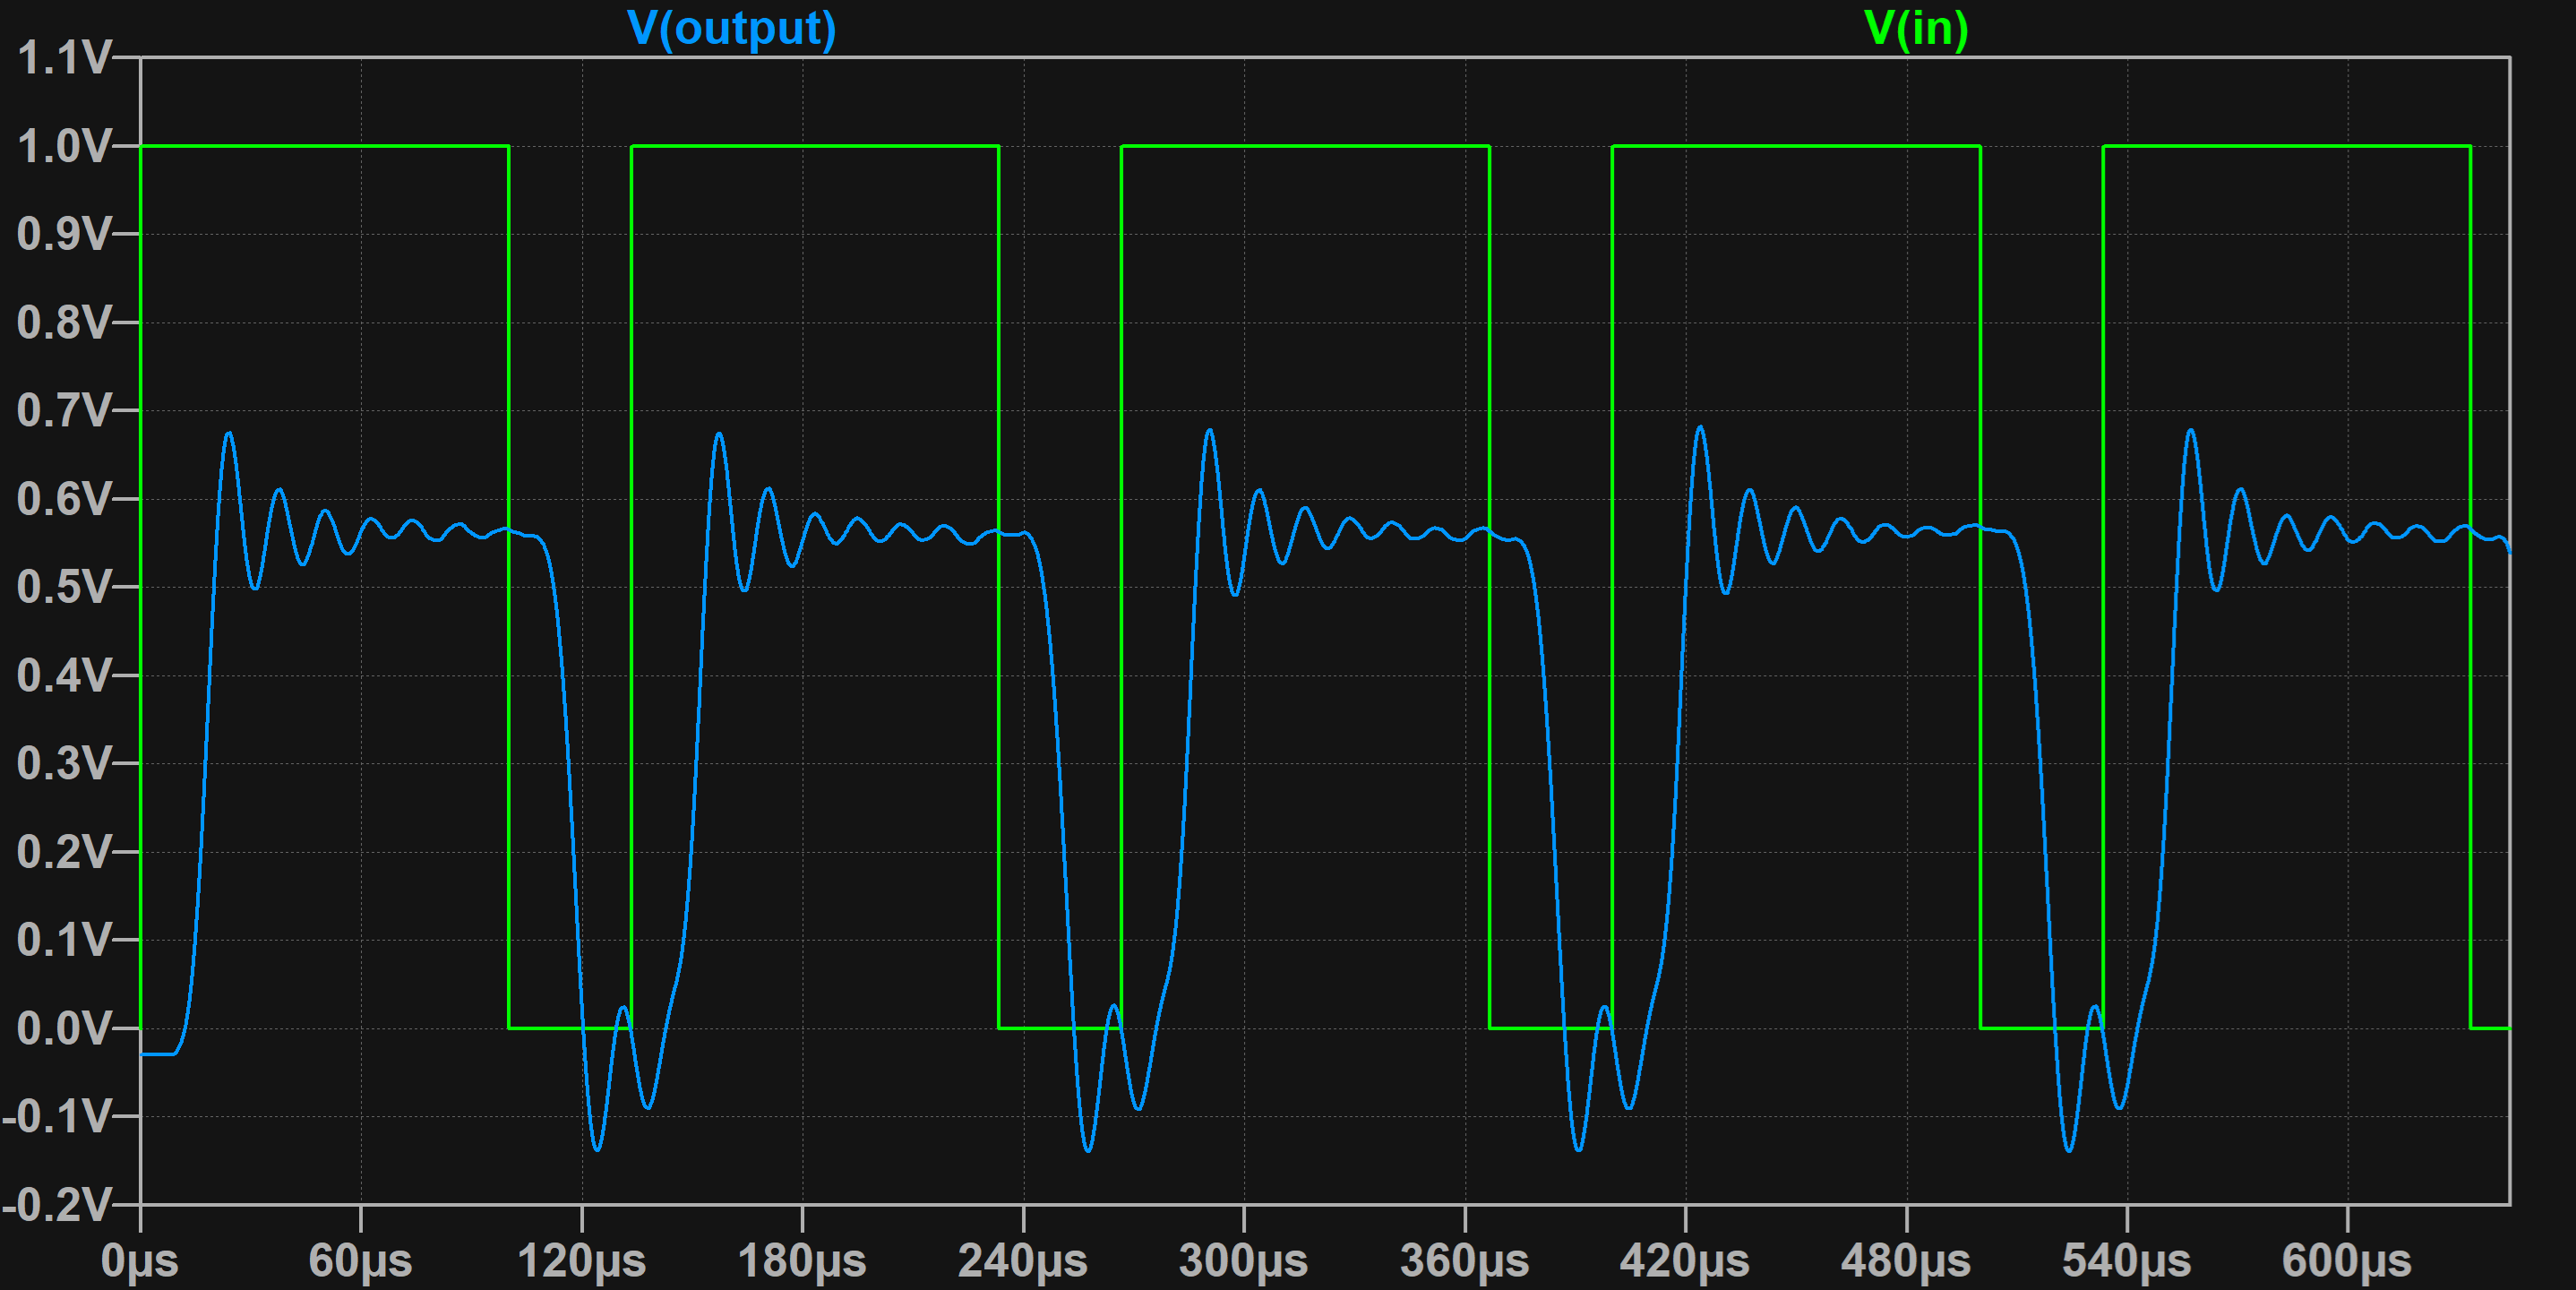
\includegraphics[width=0.8\linewidth]{Imagenes Nacho/Instantaneo/Vi-Vo.png}
    \caption{$V_o$ vs $V_i$}
    \label{fig:Vi-Vo}
\end{figure}

\begin{figure}[H]
    \centering
    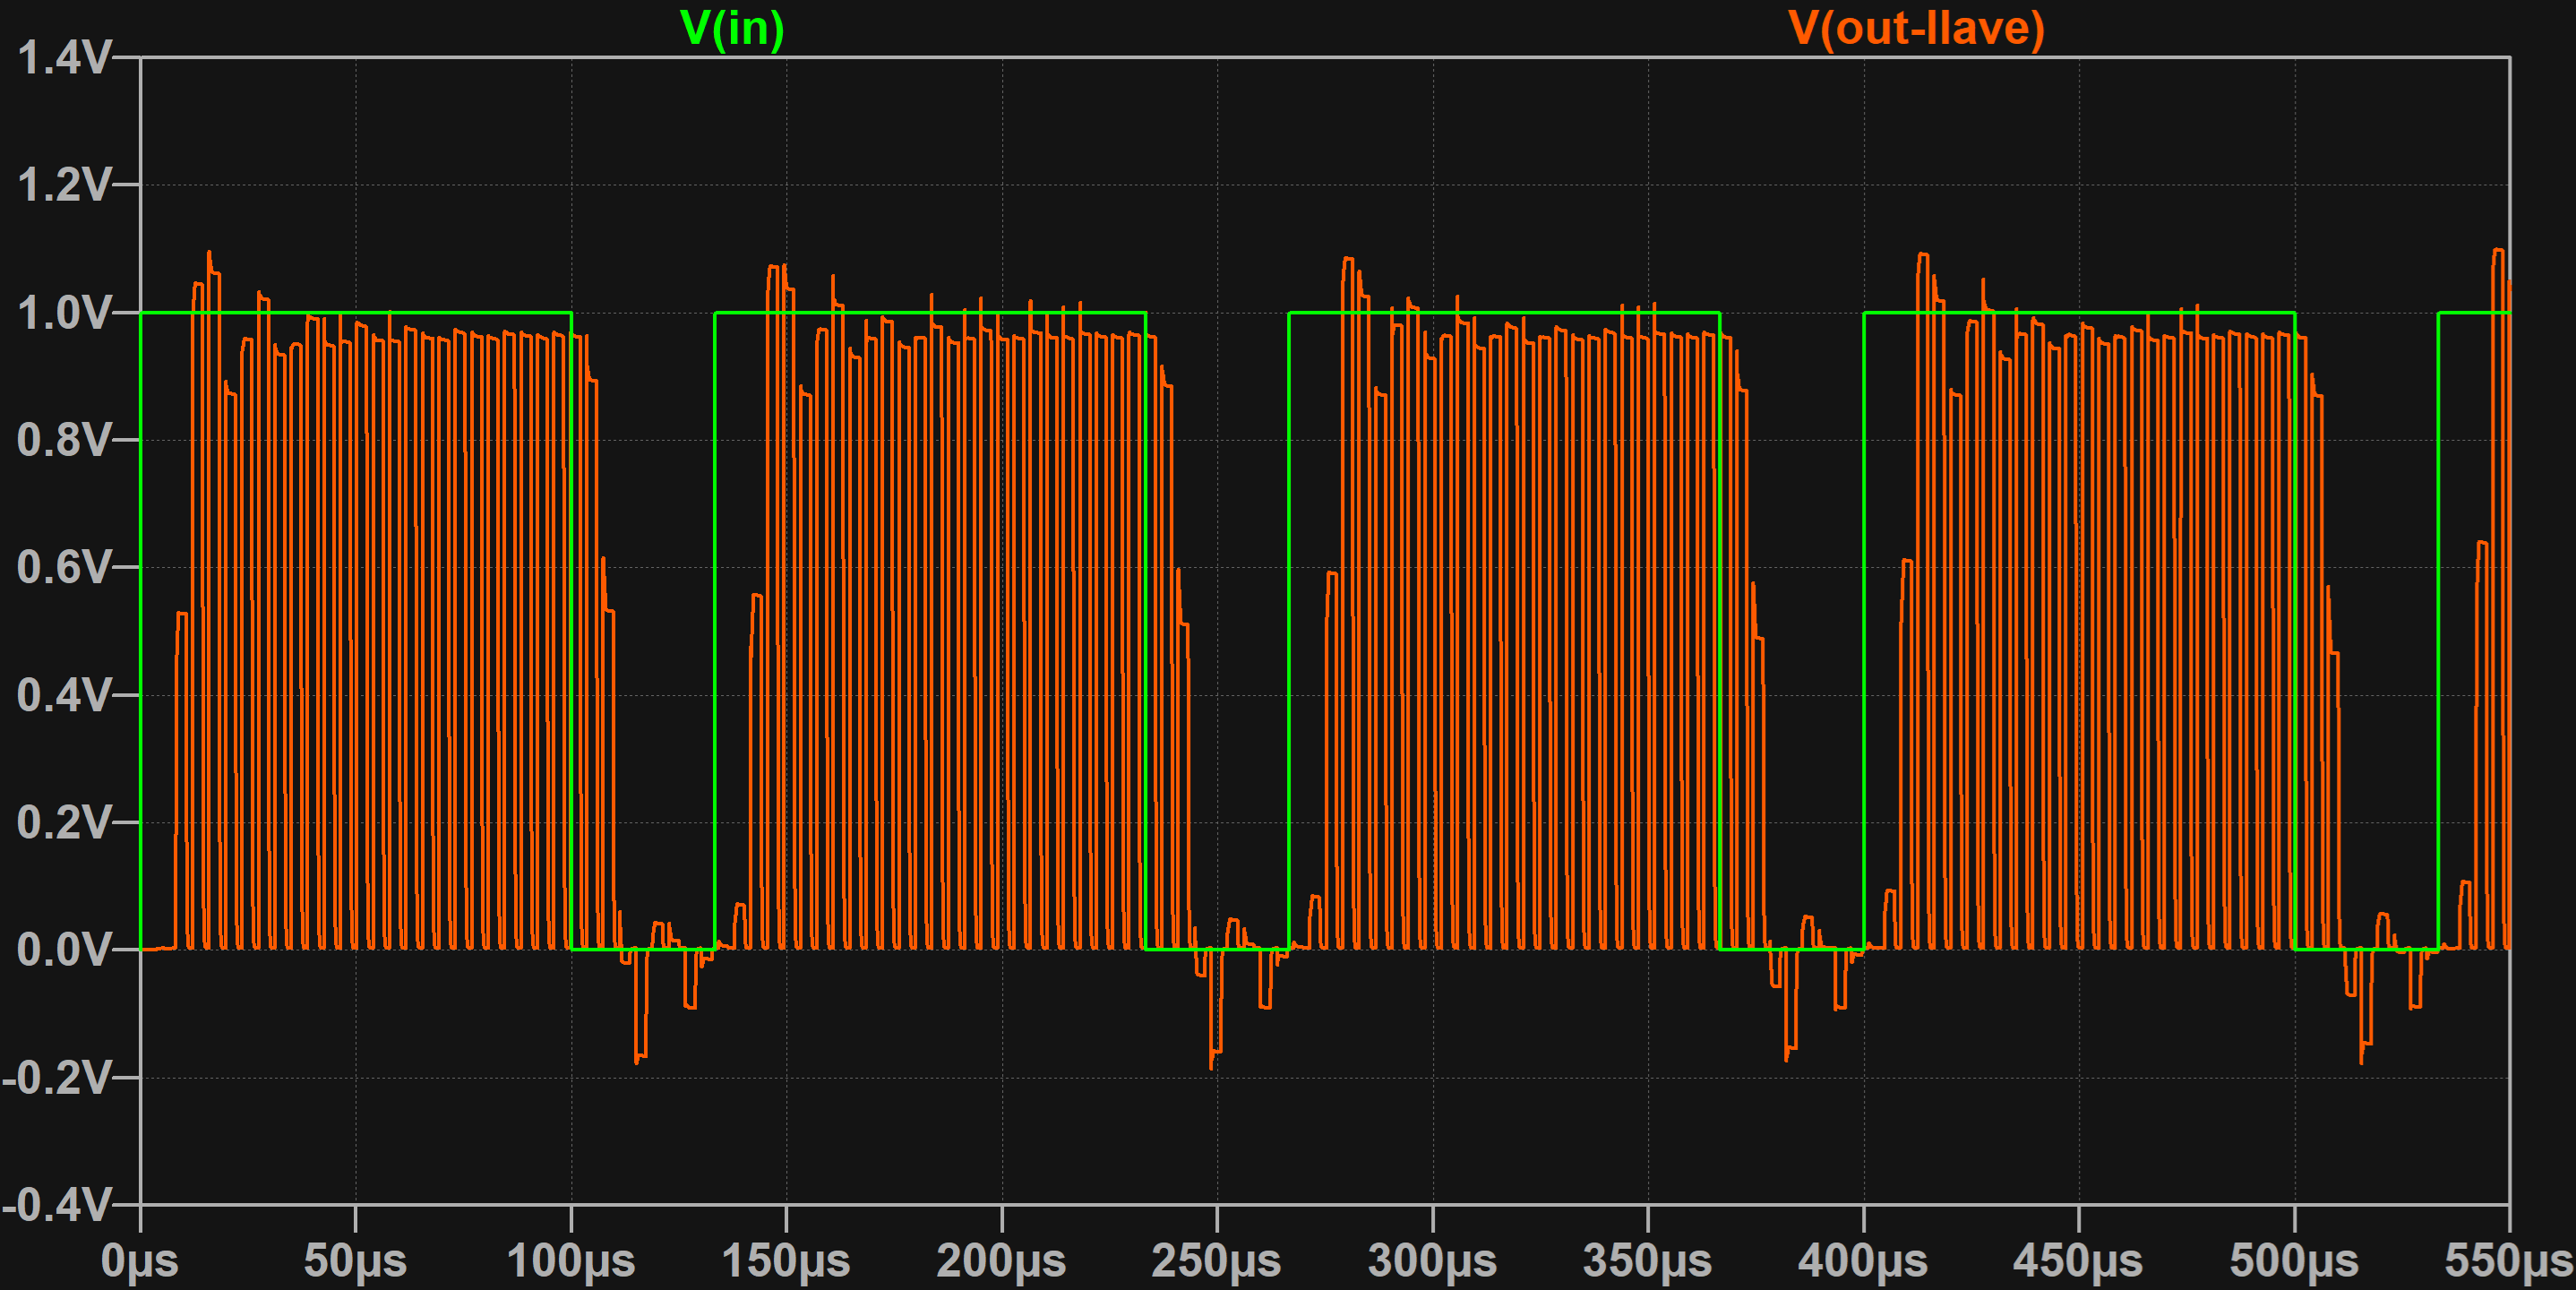
\includegraphics[width=0.8\linewidth]{Imagenes Nacho/Instantaneo/out-llave.png}
    \caption{Salida de la llave vs $V_i$}
    \label{fig:out-llave}
\end{figure}


\begin{figure}[H]
    \centering
    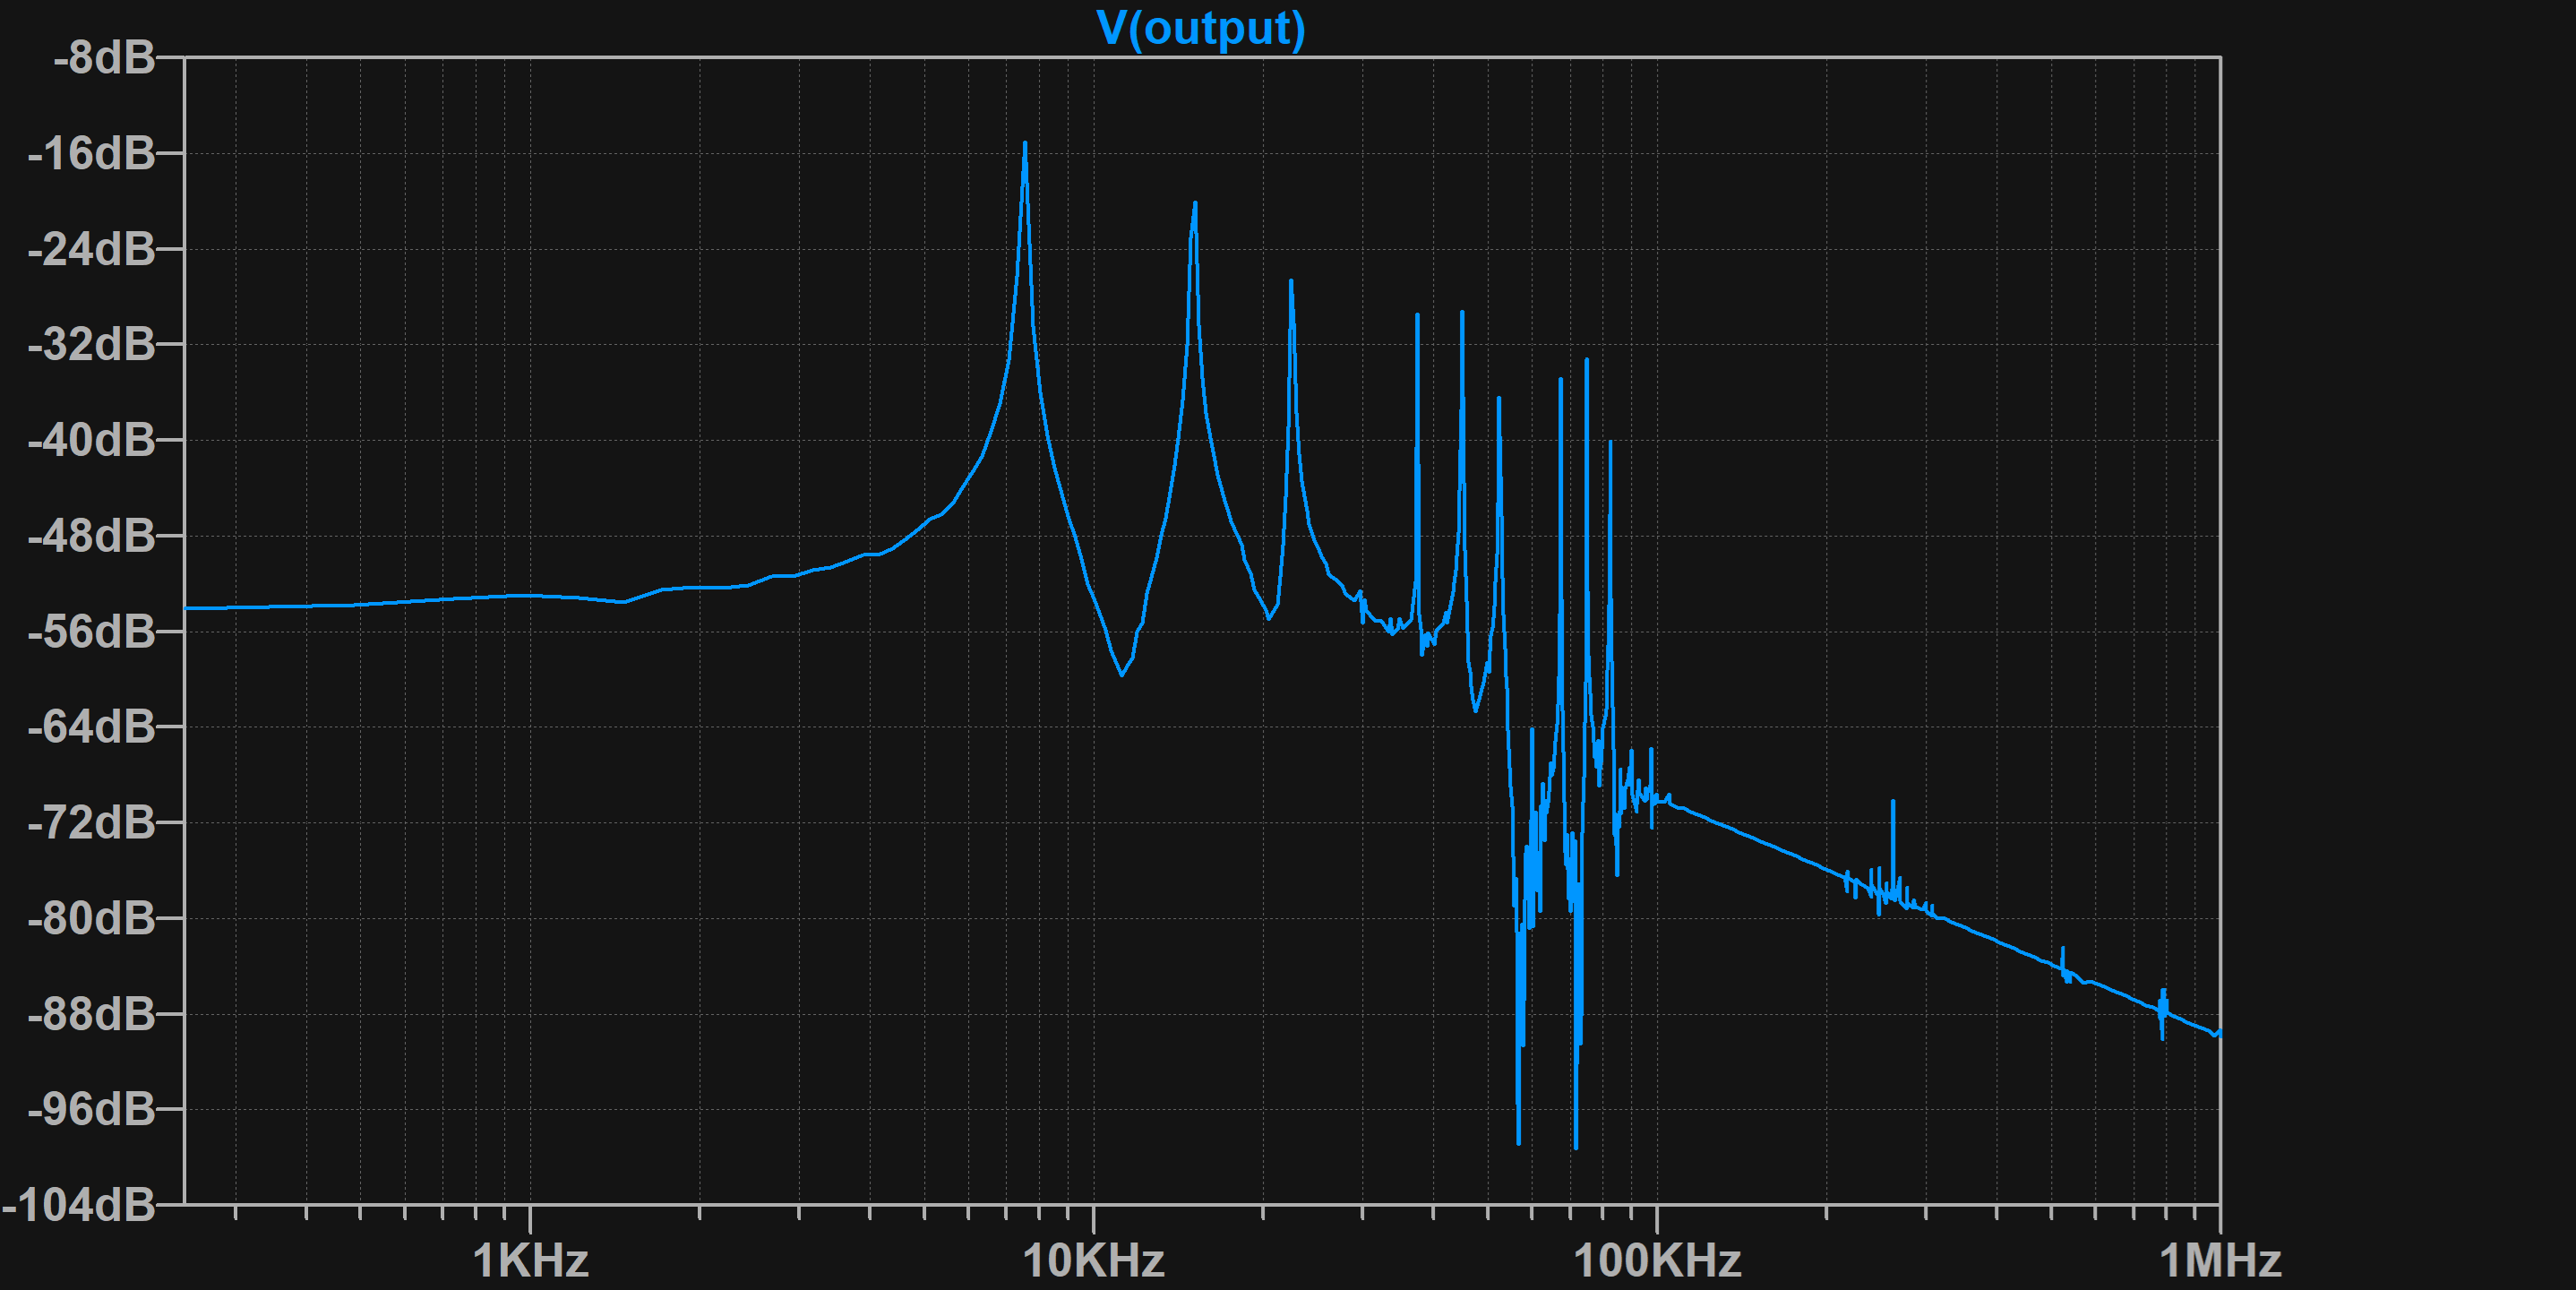
\includegraphics[width=0.8\linewidth]{Imagenes Nacho/Instantaneo/Vo-FFT.png}
    \caption{FFT de $V_o$}
    \label{fig:FFT}
\end{figure}



%---------------- 4ta Seccion ----------------%
\section{Simulaciones}
Se implemento una simulación en Python para observar los efectos del muestreo
instantáneo y natural sobre señales analógicas. El código desarrollado permite
observar que sucede en cada etapa del proceso de muestreo, ademas de tener
la capacidad de poder saltear etapas y observar los efectos de cada una, tanto 
en el dominio del tiempo como en el de la frecuencia.

El código se implemento en Python utilizando las librerías numpy, scipy, matplotlib,
y PyQt5. La interfaz gráfica permite decidir con que señal de entrada se quiere
trabajar, la frecuencia de muestreo, el tipo de muestreo (instantáneo o natural),
y la frecuencia de corte de los filtro anti-alias y de reconstrucción.
Tabién permite variar el duty cycle del sample and hold.
Ambos filtros (anti-alias y de reconstrucción) se implenetaron
usando la funcion de aproximación de Cauer (elliptic) de orden 6,
al igual que en la placa del circuito impreso.
Además, indica con puntos naranjas donde se muestreó la señal de entrada
A continuación se muestran algunas capturas de pantalla de la interfaz gráfica:

\begin{figure}[H]
    \centering
    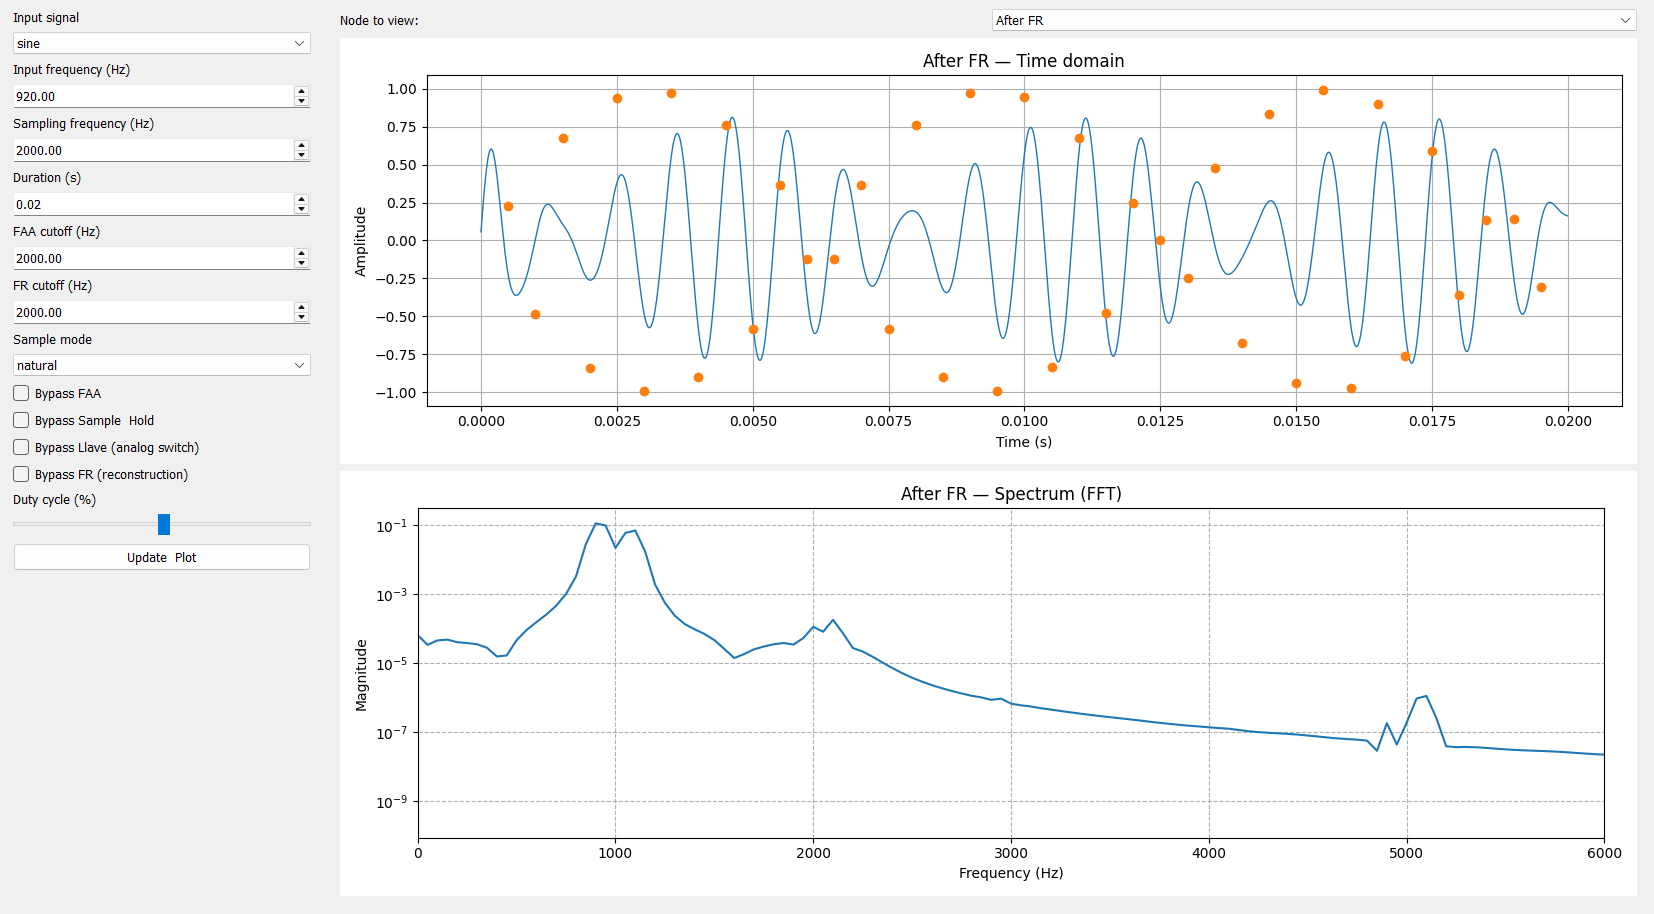
\includegraphics[width=0.8\textwidth]{Imagenes/gui_beating.png}
    \caption{Interfaz gráfica - Ejemplo de señal en la GUI}
    \label{fig:interfaz1}
\end{figure}

Donde se puede apreciar el efecto de ``beating'' ya que el la señal de entrada
es cercana a $f_s/2$, el filtro recuperador no es capaz de eliminar el aliasing
y se observa una señal modulada en amplitud.




%---------------- 5ta Seccion ----------------%
\section{Simulaciones en Python}
\input{Secciones/seccion5}

%----------------- Conclusión ----------------%
\section{Conclusión}
En esta práctica se logró implementar y analizar un sistema 
completo de muestreo de señales analógicas, incluyendo las 
modalidades ideal, natural e instantánea (Zero-Order Hold). 
A través de la combinación de simulaciones en Python, LTSpice y 
la implementación en placa, se pudo observar de manera comparativa cómo 
cada tipo de muestreo afecta la señal y su espectro en frecuencia.

Se verificó experimentalmente el Teorema de Nyquist-Shannon, 
confirmando que la frecuencia de muestreo debe ser al menos el 
doble de la frecuencia máxima de la señal para evitar aliasing. 
Además, se evidenció la importancia de los filtros anti-aliasing y 
de reconstrucción, ya que su correcta implementación permite preservar 
la mayor cantidad de armónicos de la señal original, garantizando una 
reconstrucción fiel.


En conclusión, esta experiencia permitió consolidar conceptos teóricos de muestreo, 
procesamiento de señales y filtrado, y desarrollar habilidades prácticas para 
diseñar y analizar sistemas de adquisición de señales analógicas en un entorno 
tanto simulado como real.

%---------------- Anexo ----------------%
\section{Anexo}
Repositorio del código:

https://github.com/ramibelsito/ASSD---Simulador-de-Muestreo

%---------------- Bibliografía ----------------%
\printbibliography

%---------------- Componentes ----------------%
%\newpage
%\section{Templates}
%% -------- TABLAS ---------------
\subsection{Tablas}
\begin{table}[H]
    \centering
    \begin{tabular}{l|c|c} \hline
     Columna 0 & Columna 1 & Columna 2  \\ \hline
    0 & 1 & 2  \\ 
    0 & 1 & 2 \\ \hline
    \end{tabular}
    \caption{Pie de tabla}
    \label{tab:tabla simple}
\end{table}



% ---------- FOTOS --------------
\subsection{Fotos}
% 1. Simple
\subsubsection{Foto Simple}
\begin{figure}[H]
    \centering
    \includegraphics[width=0.5\linewidth]{example-image}
    \caption{Foto simple}
    \label{fig:foto simple}
\end{figure}

% 2. Varias horizontales
\subsubsection{Fotos Horizontales}
\begin{figure}[H]
    \subfigure[Foto 1]{
    \includegraphics[width=0.3\textwidth]{example-image}}
    \subfigure[Foto 2]{
    \includegraphics[width = 0.3\textwidth]{example-image}}
    \subfigure[Foto 3]{
    \includegraphics[width = 0.3\textwidth]{example-image}}
    \label{fig:multi Fotos}
\end{figure}

% 3. Varias verticales
\subsubsection{Fotos Verticales}
\begin{figure}[H]
    \centering
    \includegraphics[width=0.5\linewidth]{example-image}
    \includegraphics[width=0.5\linewidth]{example-image}
    \caption{2 fotos verticales}
    \label{fig:fotos verticales}
\end{figure}

% 4. Grilla de Fotos
\subsubsection{Fotos en grilla}
\begin{figure}[H]
        \subfloat[Caption 1]{
            \includegraphics[width=.48\linewidth]{example-image}
            \label{subfig:a}
        }\hfill
        \subfloat[Caption 2]{
            \includegraphics[width=.48\linewidth]{example-image}
            \label{subfig:b}
        }\\
        \subfloat[Caption 3]{
            \includegraphics[width=.48\linewidth]{example-image}
            \label{subfig:c}
        }\hfill
        \subfloat[Caption 4]{
            \includegraphics[width=.48\linewidth]{example-image}
            \label{subfig:d}
        }
        \caption{Caption}
        \label{fig: grilla de fotos}
    \end{figure}

% -------------- Texto en dos columnas -------------
\subsection{Texto en Columnas}
\setlength{\columnsep}{1cm}
\begin{multicols}{2}
Lorem ipsum dolor sit amet, consectetur adipiscing elit. Proin tristique aliquam sapien pellentesque viverra. Proin in ex libero. Etiam cursus et metus ut porttitor. Nunc sit amet rhoncus velit. Nunc eu pharetra sapien. In ultricies tellus a sapien placerat, quis commodo sem consequat. Sed non felis sagittis, maximus felis dictum, scelerisque eros. Nunc in aliquet lacus. Ut consectetur odio purus. Integer sed erat quis mi vulputate molestie. Etiam viverra sapien tincidunt turpis pulvinar blandit. Nullam pharetra bibendum ligula, vitae dictum est sagittis ut. Suspendisse convallis commodo diam at elementum.
\end{multicols}

% ------------ Ecuaciones -----------------------

% Sistema de ecuaciones
\subsection{Ecuaciones}
\begin{equation}
    \begin{cases}
        2x+y=1 \\
        y+2=3
    \end{cases} \longrightarrow x=0 \wedge y=1
\end{equation} 


% Ecuaciones alineadas
\begin{equation}
    \begin{gathered}
        H(s) = \frac{1}{\frac{1}{sRC}} \\
        H(s)= sRC
    \end{gathered}
\end{equation}

% Ecuaciones alineadas por el igual
\begin{equation}
    \begin{split}
        H(s) &= \frac{1}{\frac{1}{sRC}} \\
             &= sRC
    \end{split}
\end{equation}



% Ecuaciones sin número
$$H(s)= sRC$$




% ---------------- Citas y Links -----------------
\subsection{Citas y Links}

Dirac dijo esto. \cite{dirac}

\href{http://www.overleaf.com}{Esto tiene un hipervínculo}


% ----------------- Bloque de código -------------------
\subsection{Código}
\begin{lstlisting}
# Bloque de codigo
...
...
print('Hello World!)
\end{lstlisting}





\end{document}
